%%%%%%%%%%%%%%%%%%%%%%%%%%%%%%%%%%%%
% Slide options
%%%%%%%%%%%%%%%%%%%%%%%%%%%%%%%%%%%%

% Option 1: Slides with solutions

\documentclass[slidestop,compress,mathserif]{beamer}
\newcommand{\soln}[1]{\textit{#1}}
\newcommand{\solnGr}[1]{#1}

% Option 2: Handouts without solutions

%\documentclass[11pt,containsverbatim,handout]{beamer}
%\usepackage{pgfpages}
%\pgfpagesuselayout{4 on 1}[letterpaper,landscape,border shrink=5mm]
%\newcommand{\soln}[1]{ }
%\newcommand{\solnGr}{ }

%%%%%%%%%%%%%%%%%%%%%%%%%%%%%%%%%%%%
% Style
%%%%%%%%%%%%%%%%%%%%%%%%%%%%%%%%%%%%

\input{../lec_style.tex}


%%%%%%%%%%%%%%%%%%%%%%%%%%%%%%%%%%%%
% Preamble
%%%%%%%%%%%%%%%%%%%%%%%%%%%%%%%%%%%%

\title[Chp 9: Multiple and logistic regression]{Chapter 9: Multiple and logistic regression}
\author{OpenIntro Statistics, 4th Edition}
\institute{$\:$ \\ {\footnotesize Slides developed by Mine \c{C}etinkaya-Rundel of OpenIntro. \\
The slides may be copied, edited, and/or shared via the \webLink{http://creativecommons.org/licenses/by-sa/3.0/us/}{CC BY-SA license.} \\
Some images may be included under fair use guidelines (educational purposes).}}
\date{}


%%%%%%%%%%%%%%%%%%%%%%%%%%%%%%%%%%%%
% Begin document
%%%%%%%%%%%%%%%%%%%%%%%%%%%%%%%%%%%%

\begin{document}


%%%%%%%%%%%%%%%%%%%%%%%%%%%%%%%%%%%%
% Title page
%%%%%%%%%%%%%%%%%%%%%%%%%%%%%%%%%%%%

{
\addtocounter{framenumber}{-1} 
{\removepagenumbers 
\usebackgroundtemplate{\includegraphics[width=\paperwidth]{../OpenIntro_Grid_4_3-01.jpg}}
\begin{frame}

\hfill \includegraphics[width=20mm]{../oiLogo_highres}

\titlepage

\end{frame}
}
}


%%%%%%%%%%%%%%%%%%%%%%%%%%%%%%%%%%%%
% Sections
%%%%%%%%%%%%%%%%%%%%%%%%%%%%%%%%%%%%

%%%%%%%%%%%%%%%%%%%%%%%%%%%%%%%%%%%%

\section{Introduction to multiple regression}

%%%%%%%%%%%%%%%%%%%%%%%%%%%%%%%%%%%%

\begin{frame}
\frametitle{Multiple regression}

\begin{itemize}

\item Simple linear regression: Bivariate - two variables: $y$ and $x$

\item Multiple linear regression: Multiple variables: $y$ and $x_1, x_2, \cdots$

\end{itemize}

\end{frame}

%%%%%%%%%%%%%%%%%%%%%%%%%%%%%%%%%%%%

\subsection{Many variables in a model}

%%%%%%%%%%%%%%%%%%%%%%%%%%%%%%%%%%%%

\begin{frame}
\frametitle{Weights of books}

\twocol{0.6}{0.4}{
{\small
\begin{center}
\begin{tabular}{rrrc}
  \hline
 & weight (g) & volume (cm$^\text{3}$) & cover \\ 
  \hline
1 & 800 & 885 & hc \\ 
  2 & 950 & 1016 & hc \\ 
  3 & 1050 & 1125 & hc \\ 
  4 & 350 & 239 & hc \\ 
  5 & 750 & 701 & hc \\ 
  6 & 600 & 641 & hc \\ 
  7 & 1075 & 1228 & hc \\ 
  8 & 250 & 412 & pb \\ 
  9 & 700 & 953 & pb \\ 
  10 & 650 & 929 & pb \\ 
  11 & 975 & 1492 & pb \\ 
  12 & 350 & 419 & pb \\ 
  13 & 950 & 1010 & pb \\ 
  14 & 425 & 595 & pb \\ 
  15 & 725 & 1034 & pb \\ 
   \hline
\end{tabular}
\end{center}
}}
{
\begin{center}
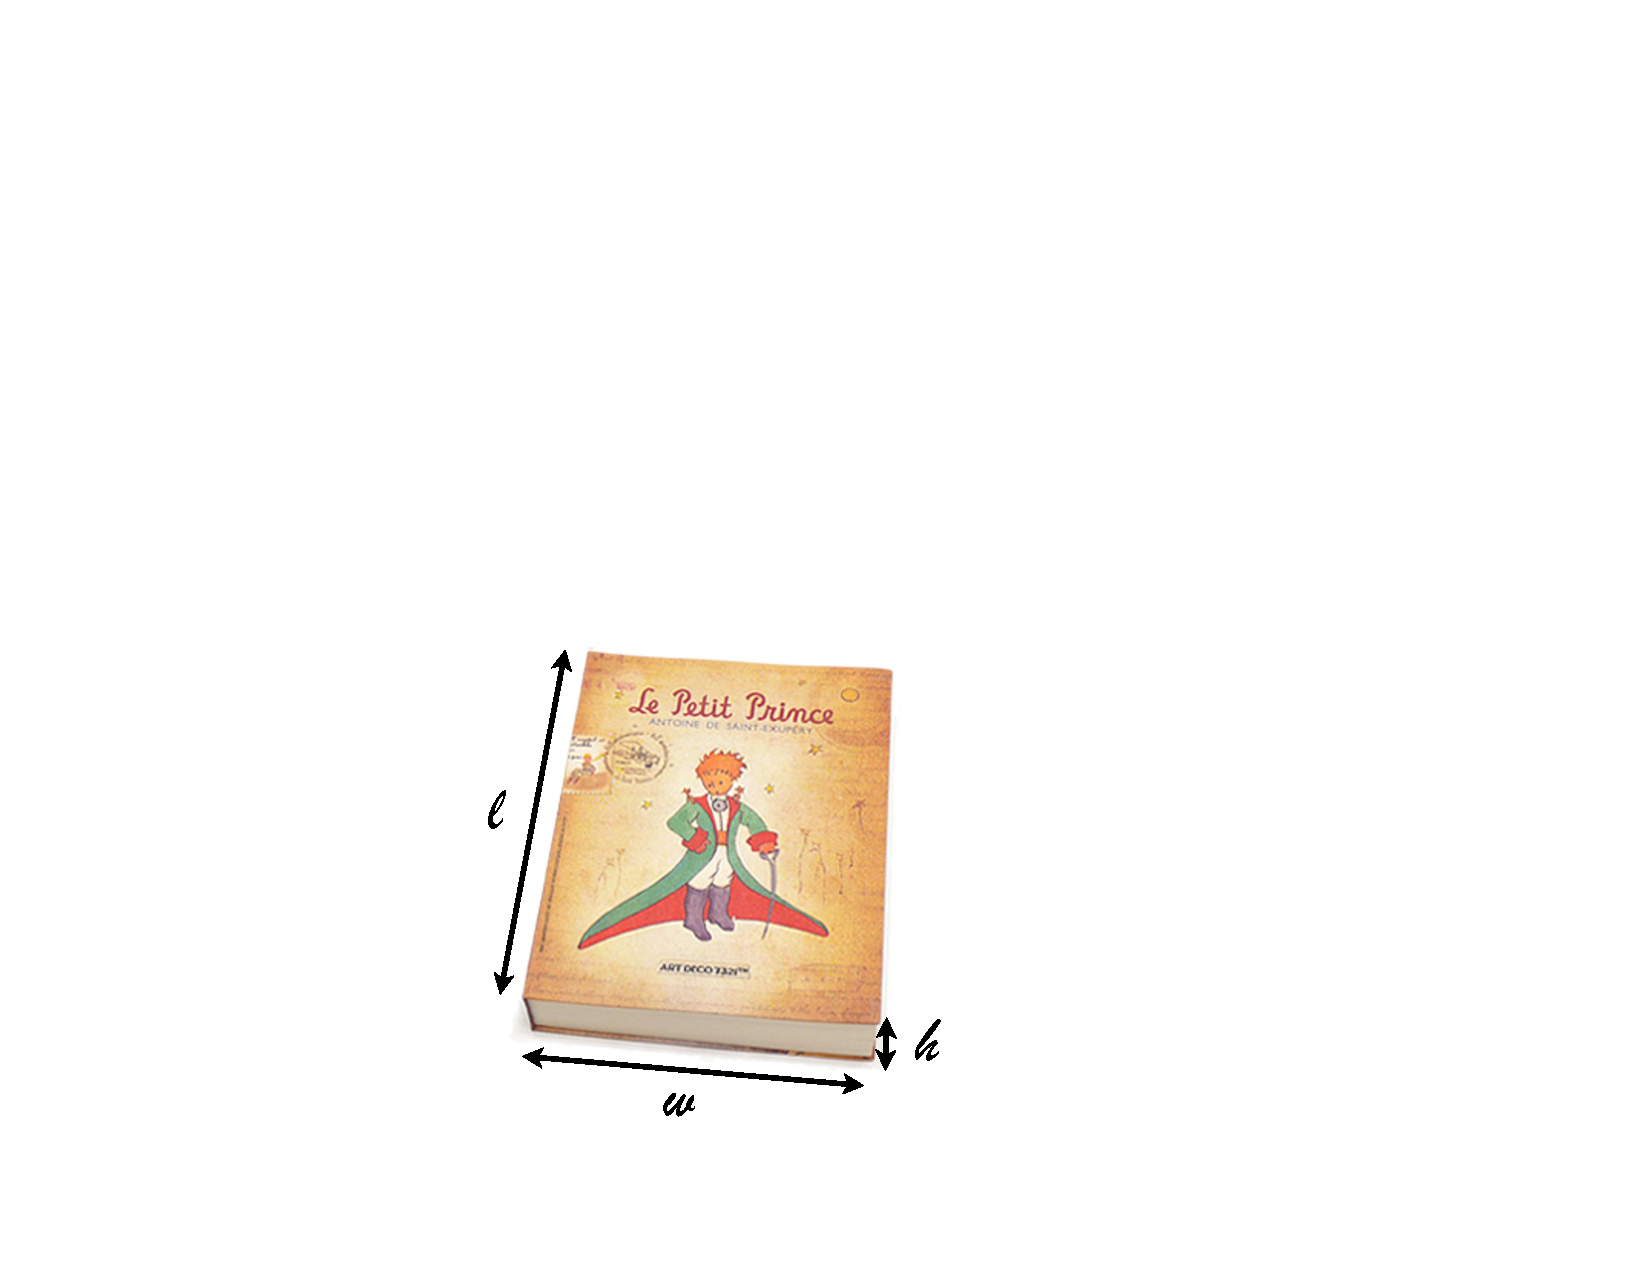
\includegraphics[width=0.7\textwidth]{9-1_intro_mlr/figures/books/book}
\end{center}
}

\ct{From: Maindonald, J.H. and Braun, W.J. (2nd ed., 2007) ``Data Analysis and Graphics Using R"}

\end{frame}

%%%%%%%%%%%%%%%%%%%%%%%%%%%%%%%%%%%

\begin{frame}
\frametitle{Weights of books (cont.)}

\twocol{0.45}{0.45}
{
\pq{{\small The scatterplot shows the relationship between weights and volumes of books as well as the regression output. Which of the below is correct?}}
}
{
\begin{center}
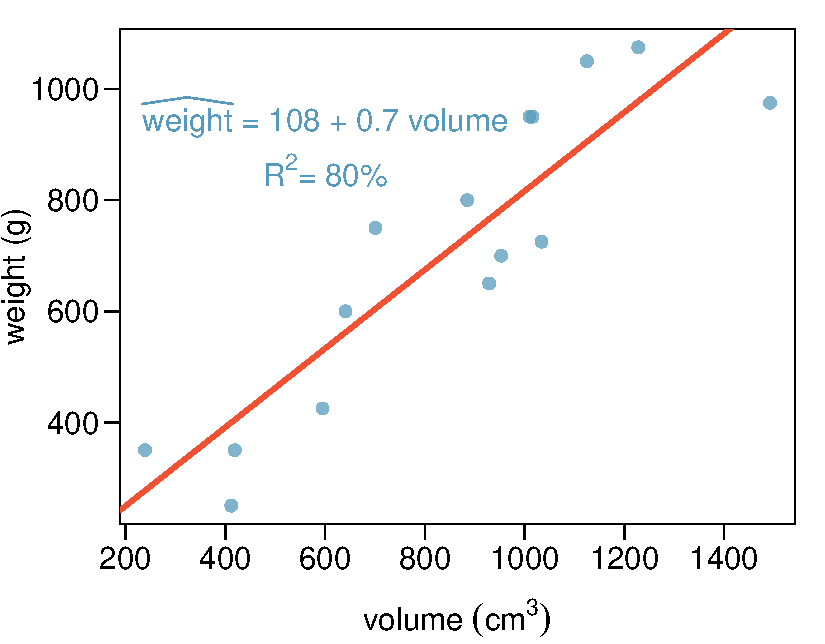
\includegraphics[width=\textwidth]{9-1_intro_mlr/figures/books/weight_volume}
\end{center}
}

\begin{enumerate}[(a)]
\item Weights of 80\% of the books can be predicted accurately using this model.
\solnMult{Books that are 10 cm$^\text{3}$ over average are expected to weigh 7 g over average.}
\item The correlation between weight and volume is $R = 0.80^2 = 0.64$.
\item The model underestimates the weight of the book with the highest volume.
\end{enumerate}

\end{frame}

%%%%%%%%%%%%%%%%%%%%%%%%%%%%%%%%%%%

\begin{frame}[fragile]
\frametitle{Modeling weights of books using volume}

{\small \textit{somewhat abbreviated output...}}

\begin{verbatim}
Coefficients:
             Estimate Std. Error t value Pr(>|t|)    
(Intercept) 107.67931   88.37758   1.218    0.245    
volume        0.70864    0.09746   7.271 6.26e-06


Residual standard error: 123.9 on 13 degrees of freedom
Multiple R-squared: 0.8026,	Adjusted R-squared: 0.7875 
F-statistic: 52.87 on 1 and 13 DF,  p-value: 6.262e-06 
\end{verbatim}

\end{frame}

%%%%%%%%%%%%%%%%%%%%%%%%%%%%%%%%%%%

\begin{frame}
\frametitle{Weights of hardcover and paperback books}

\dq{Can you identify a trend in the relationship between volume and weight of hardcover and paperback books?}

\soln{\only<2>{{\small Paperbacks generally weigh less than hardcover books after controlling for the book?s volume.}}}

\begin{center}
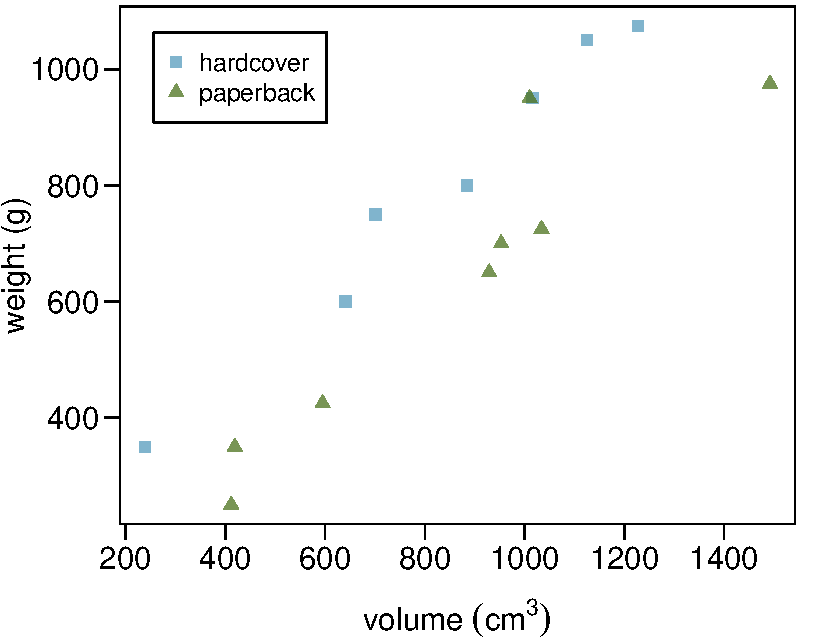
\includegraphics[width=0.6\textwidth]{9-1_intro_mlr/figures/books/weight_volume_cover}
\end{center}

\end{frame}

%%%%%%%%%%%%%%%%%%%%%%%%%%%%%%%%%%%

\begin{frame}[fragile]
\frametitle{Modeling weights of books using volume \underline{and} cover type}

\begin{verbatim}
Coefficients:
              Estimate Std. Error t value Pr(>|t|)    
(Intercept)  197.96284   59.19274   3.344 0.005841 ** 
volume         0.71795    0.06153  11.669  6.6e-08 ***
cover:pb    -184.04727   40.49420  -4.545 0.000672 ***


Residual standard error: 78.2 on 12 degrees of freedom
Multiple R-squared: 0.9275,	Adjusted R-squared: 0.9154 
F-statistic: 76.73 on 2 and 12 DF,  p-value: 1.455e-07 
\end{verbatim}

\end{frame}

%%%%%%%%%%%%%%%%%%%%%%%%%%%%%%%%%%%

\begin{frame}
\frametitle{Determining the reference level}

\pq{Based on the regression output below, which level of \var{cover} is the reference level? Note that \var{pb}: paperback.}

{\small
\begin{center}
\begin{tabular}{rrrrr}
  \hline
 & Estimate & Std. Error & t value & Pr($>$$|$t$|$) \\ 
  \hline
(Intercept) & 197.9628 & 59.1927 & 3.34 & 0.0058 \\ 
  volume & 0.7180 & 0.0615 & 11.67 & 0.0000 \\ 
  cover:pb & -184.0473 & 40.4942 & -4.55 & 0.0007 \\ 
   \hline
\end{tabular}
\end{center}
}

\begin{enumerate}[(a)]
\item paperback
\solnMult{hardcover}
\end{enumerate}

\end{frame}

%%%%%%%%%%%%%%%%%%%%%%%%%%%%%%%%%%%

\begin{frame}
\frametitle{Determining the reference level}

\pq{Which of the below correctly describes the roles of variables in this regression model?}

{\small
\begin{center}
\begin{tabular}{rrrrr}
  \hline
 & Estimate & Std. Error & t value & Pr($>$$|$t$|$) \\ 
  \hline
(Intercept) & 197.9628 & 59.1927 & 3.34 & 0.0058 \\ 
  volume & 0.7180 & 0.0615 & 11.67 & 0.0000 \\ 
  cover:pb & -184.0473 & 40.4942 & -4.55 & 0.0007 \\ 
   \hline
\end{tabular}
\end{center}
}

\begin{enumerate}[(a)]
\item response: weight, explanatory: volume, paperback cover
\item response: weight, explanatory: volume, hardcover cover
\item response: volume, explanatory: weight, cover type
\solnMult{response: weight, explanatory: volume, cover type}
\end{enumerate}

\end{frame}

%%%%%%%%%%%%%%%%%%%%%%%%%%%%%%%%%%%

\begin{frame}
\frametitle{Linear model}

{\small
\begin{center}
\begin{tabular}{rrrrr}
  \hline
 & Estimate & Std. Error & t value & Pr($>$$|$t$|$) \\ 
  \hline
(Intercept) & 197.96 & 59.19 & 3.34 & 0.01 \\ 
  volume & 0.72 & 0.06 & 11.67 & 0.00 \\ 
  cover:pb & -184.05 & 40.49 & -4.55 & 0.00 \\ 
   \hline
\end{tabular}
\end{center}
}

\pause

\[ \widehat{weight} = 197.96 + 0.72~volume - 184.05~cover:pb  \]

\pause

\begin{enumerate}

\item For \hl{hardcover} books: plug in \orange{0} for \var{cover}
\begin{eqnarray*}
\widehat{weight} &=& 197.96 + 0.72~volume - 184.05 \times \orange{0} \\
\pause
&=& 197.96 +  0.72~volume
\end{eqnarray*}

\pause

\item For \orange{paperback} books: plug in \orange{1} for \var{cover}
\begin{eqnarray*}
\widehat{weight} &=& 197.96 + 0.72~volume - 184.05 \times \orange{1} \\
\pause
&=& 13.91 +  0.72~volume
\end{eqnarray*}

\end{enumerate}

\end{frame}

%%%%%%%%%%%%%%%%%%%%%%%%%%%%%%%%%%%

\begin{frame}
\frametitle{Visualising the linear model}

\begin{center}
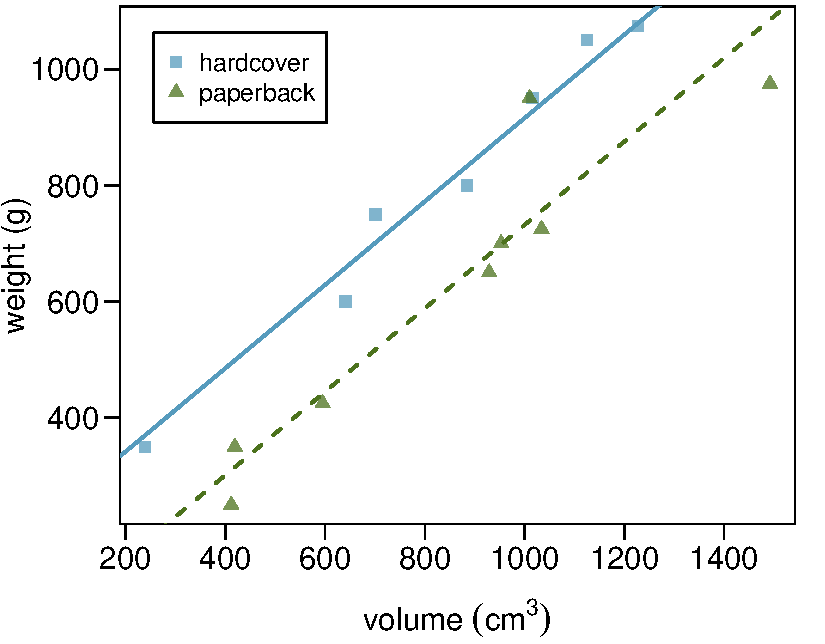
\includegraphics[width=0.8\textwidth]{9-1_intro_mlr/figures/books/weight_volume_cover_lines}
\end{center}

\end{frame}

%%%%%%%%%%%%%%%%%%%%%%%%%%%%%%%%%%%

\begin{frame}
\frametitle{Interpretation of the regression coefficients}

{\small
\begin{center}
\begin{tabular}{rrrrr}
  \hline
 & Estimate & Std. Error & t value & Pr($>$$|$t$|$) \\ 
  \hline
(Intercept) & 197.96 & 59.19 & 3.34 & 0.01 \\ 
  volume & 0.72 & 0.06 & 11.67 & 0.00 \\ 
  cover:pb & -184.05 & 40.49 & -4.55 & 0.00 \\ 
   \hline
\end{tabular}
\end{center}
}

\pause

\begin{itemize}

\item \hl{Slope of volume:} \underline{All else held constant}, books that are 1 more cubic centimeter in volume tend to weigh about 0.72 grams more.

\pause

\item \hl{Slope of cover:} \underline{All else held constant}, the model predicts that paperback books weigh 184 grams lower than hardcover books.

\pause

\item \hl{Intercept:} Hardcover books with no volume are expected on average to weigh 198 grams. \pause
\begin{itemize}
\item Obviously, the intercept does not make sense in context. It only serves to adjust the height of the line.
\end{itemize}

\end{itemize}

\end{frame}

%%%%%%%%%%%%%%%%%%%%%%%%%%%%%%%%%%%

\begin{frame}
\frametitle{Prediction}

\pq{Which of the following is the correct calculation for the predicted weight of a paperback book that is 600 cm$^3$?}

{\small
\begin{center}
\begin{tabular}{rrrrr}
  \hline
 & Estimate & Std. Error & t value & Pr($>$$|$t$|$) \\ 
  \hline
(Intercept) & 197.96 & 59.19 & 3.34 & 0.01 \\ 
  volume & 0.72 & 0.06 & 11.67 & 0.00 \\ 
  cover:pb & -184.05 & 40.49 & -4.55 & 0.00 \\ 
   \hline
\end{tabular}
\end{center}
}

\begin{enumerate}[(a)]
\solnMult{197.96 + 0.72 * 600 - 184.05 * 1} \soln{\only<2>{\orange{~$= 445.91$ grams}}}
\item 184.05 + 0.72 * 600 - 197.96 * 1
\item 197.96 + 0.72 * 600 - 184.05 * 0
\item 197.96 + 0.72 * 1 - 184.05 * 600
\end{enumerate}

\end{frame}

%%%%%%%%%%%%%%%%%%%%%%%%%%%%%%%%%%%

\begin{frame}
\frametitle{Another example: Modeling kid's test scores}

Predicting cognitive test scores of three- and four-year-old children using characteristics of their mothers. Data are from a survey of adult American women and their children - a subsample from the National Longitudinal Survey of Youth.

{\small
\begin{center}
\begin{tabular}{rrlrlr}
  \hline
 & kid\_score & mom\_hs & mom\_iq & mom\_work & mom\_age \\ 
  \hline
1 &  65 & yes & 121.12 & yes &  27 \\ 
  \vdots \\
  5 & 115 & yes & 92.75 & yes &  27 \\ 
  6 &  98 & no & 107.90 & no &  18 \\ 
  \vdots \\
  434 &  70 & yes & 91.25 & yes &  25 \\ 
   \hline
\end{tabular}
\end{center}
}

\vfill

{\tiny Gelman, Hill. \textit{Data Analysis Using Regression and Multilevel/Hierarchical Models}. (2007) Cambridge University Press.}

\end{frame}

%%%%%%%%%%%%%%%%%%%%%%%%%%%%%%%%%%%

\begin{frame}
\frametitle{Interpreting the slope}

\dq{What is the correct interpretation of the \underline{slope for mom's IQ}?}

{\small
\begin{center}
\begin{tabular}{rrrrr}
  \hline
 & Estimate & Std. Error & t value & Pr($>$$|$t$|$) \\ 
  \hline
(Intercept) & 19.59 & 9.22 & 2.13 & 0.03 \\ 
  mom\_hs:yes & 5.09 & 2.31 & 2.20 & 0.03 \\ 
  mom\_iq & 0.56 & 0.06 & 9.26 & 0.00 \\ 
  mom\_work:yes & 2.54 & 2.35 & 1.08 & 0.28 \\ 
  mom\_age & 0.22 & 0.33 & 0.66 & 0.51 \\ 
   \hline
\end{tabular}
\end{center}
}

$\:$ \\

\soln{\only<2>{All else held constant}, kids with mothers whose IQs are one point higher tend to score on average 0.56 points higher.}

\end{frame}

%%%%%%%%%%%%%%%%%%%%%%%%%%%%%%%%%%%

\begin{frame}
\frametitle{Interpreting the slope}

\dq{What is the correct interpretation of the \underline{intercept}?}

{\small
\begin{center}
\begin{tabular}{rrrrr}
  \hline
 & Estimate & Std. Error & t value & Pr($>$$|$t$|$) \\ 
  \hline
(Intercept) & 19.59 & 9.22 & 2.13 & 0.03 \\ 
  mom\_hs:yes & 5.09 & 2.31 & 2.20 & 0.03 \\ 
  mom\_iq & 0.56 & 0.06 & 9.26 & 0.00 \\ 
  mom\_work:yes & 2.54 & 2.35 & 1.08 & 0.28 \\ 
  mom\_age & 0.22 & 0.33 & 0.66 & 0.51 \\ 
   \hline
\end{tabular}
\end{center}
}

$\:$ \\

\soln{\only<2>{Kids whose moms haven't gone to HS, did not work during the first three years of the kid's life, have an IQ of 0 and are 0 yrs old are expected on average to score 19.59. Obviously, the intercept does not make any sense in context.}}

\end{frame}

%%%%%%%%%%%%%%%%%%%%%%%%%%%%%%%%%%%

\begin{frame}
\frametitle{Interpreting the slope}

\pq{What is the correct interpretation of the slope for \var{mom\_work}?}

{\scriptsize
\begin{center}
\begin{tabular}{rrrrr}
  \hline
 & Estimate & Std. Error & t value & Pr($>$$|$t$|$) \\ 
  \hline
(Intercept) & 19.59 & 9.22 & 2.13 & 0.03 \\ 
  mom\_hs:yes & 5.09 & 2.31 & 2.20 & 0.03 \\ 
  mom\_iq & 0.56 & 0.06 & 9.26 & 0.00 \\ 
  mom\_work:yes & 2.54 & 2.35 & 1.08 & 0.28 \\ 
  mom\_age & 0.22 & 0.33 & 0.66 & 0.51 \\ 
   \hline
\end{tabular}
\end{center}
}

All else being equal, kids whose moms worked during the first three year's of the kid's life
\begin{enumerate}[(a)]
\item are estimated to score 2.54 points lower
\solnMult{are estimated to score 2.54 points higher}
\end{enumerate}
than those whose moms did not work.
 
\end{frame}

%%%%%%%%%%%%%%%%%%%%%%%%%%%%%%%%%%%

\subsection{Adjusted $R^2$}

%%%%%%%%%%%%%%%%%%%%%%%%%%%%%%%%%%%

\begin{frame}
\frametitle{Revisit: Modeling poverty}

\vspace{-0.75cm}

\begin{center}
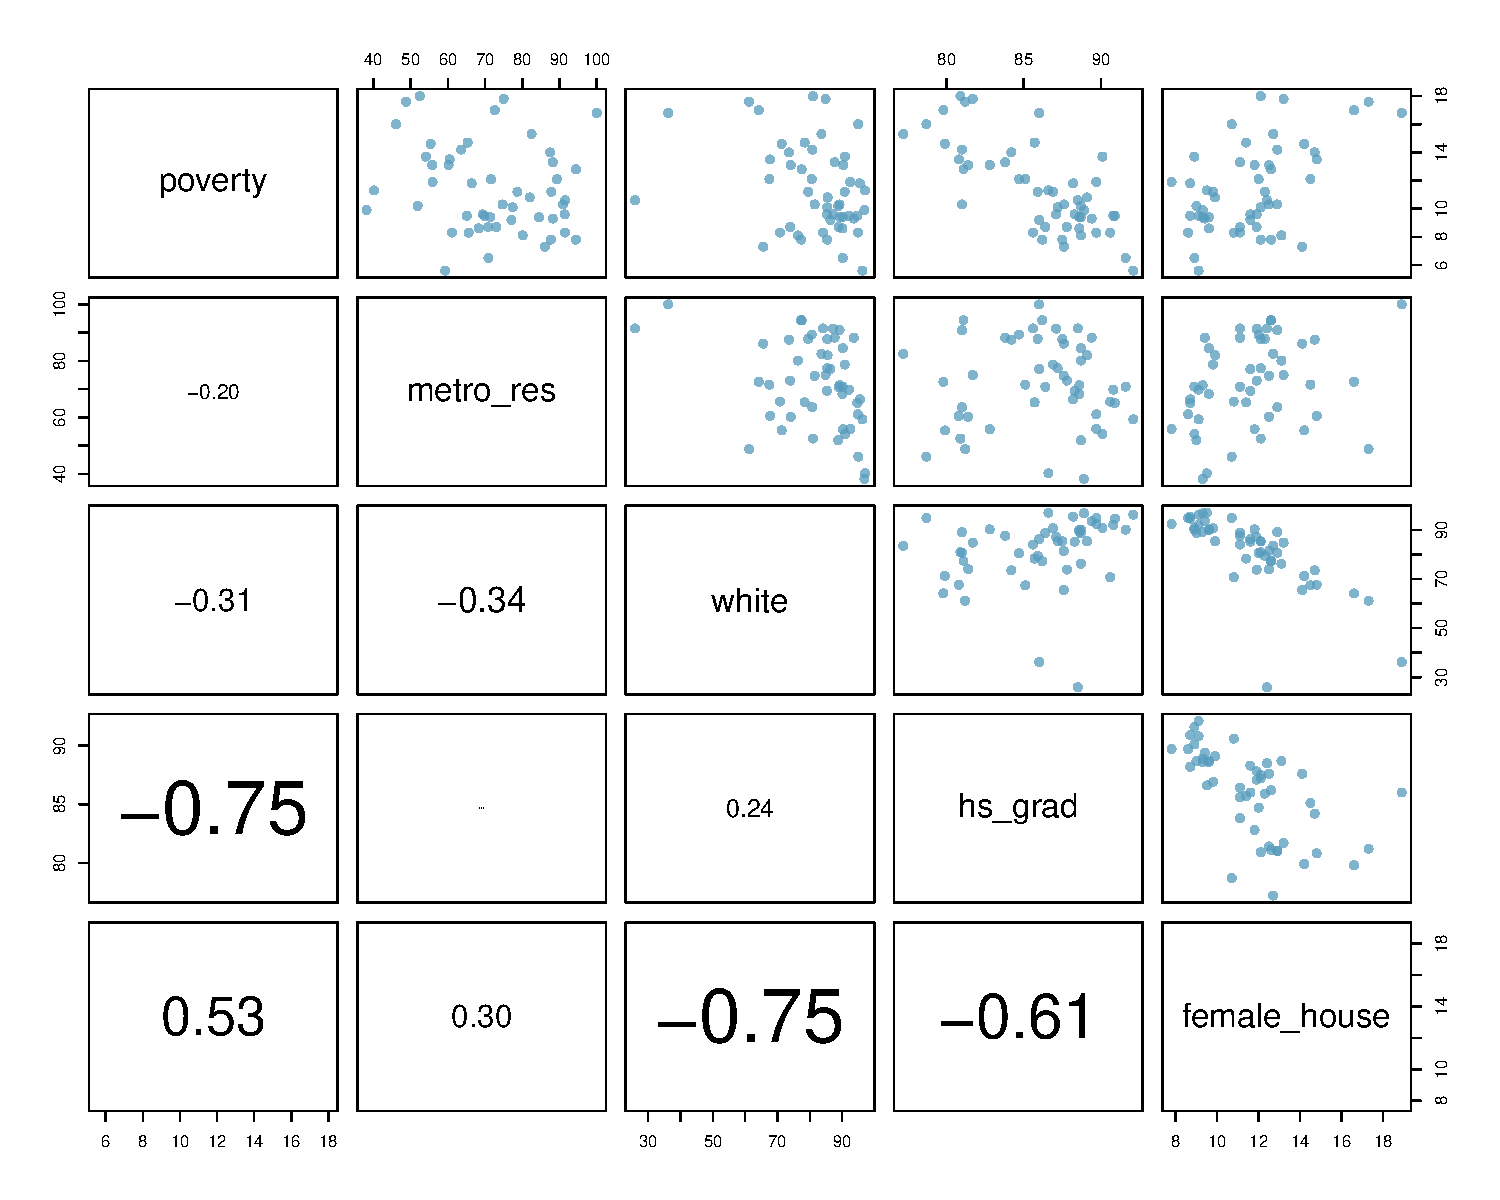
\includegraphics[width=0.9\textwidth]{9-1_intro_mlr/figures/poverty/poverty}
\end{center}

\end{frame}

%%%%%%%%%%%%%%%%%%%%%%%%%%%%%%%%%%%

\begin{frame}[fragile]
\frametitle{Predicting poverty using \% female householder}

\vspace{-0.25cm}

\begin{center}
\begin{tabular}{rrrrr}
  \hline
 & Estimate & Std. Error & t value & Pr($>$$|$t$|$) \\ 
  \hline
(Intercept) & 3.31 & 1.90 & 1.74 & 0.09 \\ 
  female\_house & 0.69 & 0.16 & 4.32 & 0.00 \\ 
   \hline
\end{tabular}
\end{center}
\twocol{0.5}{0.4}
{
\begin{center}
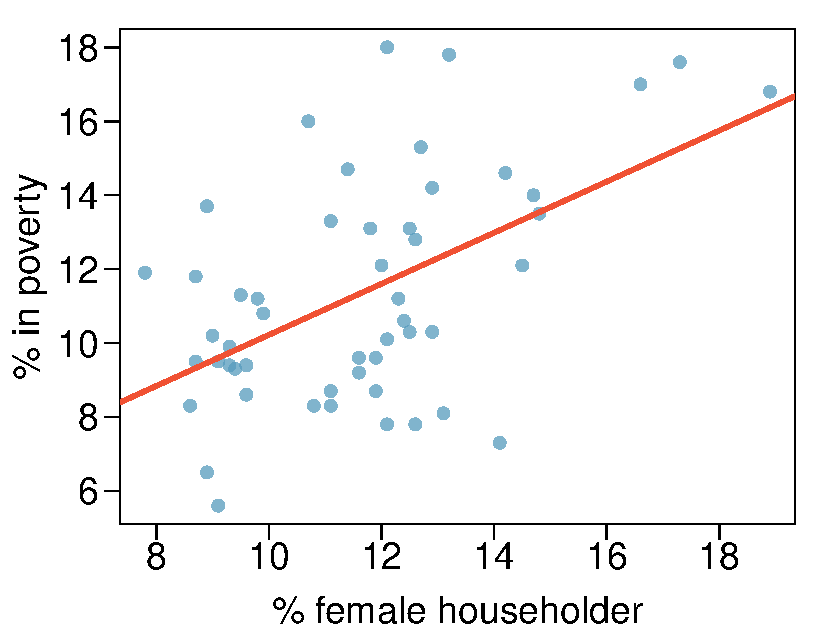
\includegraphics[width=\textwidth]{9-1_intro_mlr/figures/poverty/poverty_female_house}
\end{center}
}
{
\begin{align*}
R &= 0.53 \\
R^2 &= 0.53^2 = 0.28
\end{align*}
}

\end{frame}

%%%%%%%%%%%%%%%%%%%%%%%%%%%%%%%%%%%

\begin{frame}[fragile]
\frametitle{Another look at $R^2$}

$R^2$ can be calculated in three ways:

\pause

\begin{enumerate}

\item square the correlation coefficient of $x$ and $y$ {\small (how we have been calculating it)}

\pause

\item square the correlation coefficient of $y$ and $\hat{y}$

\pause

\item based on definition: 

\[ R^2 = \frac{\text{explained variability in }y}{\text{total variability in }y} \]

\end{enumerate}

\pause

Using \hl{ANOVA} we can calculate the explained variability and total variability in $y$.

\end{frame}


%%%%%%%%%%%%%%%%%%%%%%%%%%%%%%%%%%

\begin{frame}[fragile]
\frametitle{Sum of squares}

\vspace{-0.5cm}

{\small
\begin{center}
\begin{tabular}{lrrrrr}
  \hline
 & Df & Sum Sq & Mean Sq & F value & Pr($>$F) \\ 
  \hline
female\_house & 1 & 132.57 & 132.57 & 18.68 & 0.00 \\ 
  Residuals & 49 & 347.68 & 7.10 &  &  \\ 
   \hline
Total & 50 & 480.25 \\
   \hline
\end{tabular}
\end{center}
}

\pause

\begin{changemargin}{-1cm}{-1cm}
\begin{eqnarray*}
\text{Sum of squares of $y$: } SS_{Total} &=& \sum(y - \bar{y})^2 = 480.25 \orange{ {\footnotesize ~$\rightarrow$ total variability}} \\
\pause
%\text{Variance of $y$: } V(y) &=&  \frac{\sum(y - \bar{y})^2}{n-1} = 9.6 \\
%\pause
\text{Sum of squares of residuals: } SS_{Error} &=& \sum e_i^2 = 347.68 \orange{ { \footnotesize ~$\rightarrow$ unexplained variability}} \\
\pause
\text{Sum of squares of $x$: } SS_{Model} &=& SS_{Total} - SS_{Error} \orange{ {\footnotesize ~$\rightarrow$ explained variability}} \\
&=& 480.25 - 347.68 = 132.57
\end{eqnarray*}
\end{changemargin}

\pause

\[ R^2 = \frac{\text{explained variability}}{\text{total variability}} = \frac{132.57}{480.25} = 0.28 \green{~$\checkmark$} \]

\end{frame}

%%%%%%%%%%%%%%%%%%%%%%%%%%%%%%%%%%

\begin{frame}
\frametitle{Why bother?}

\dq{Why bother with another approach for calculating $R^2$ when we had a perfectly good way to calculate it as the correlation coefficient squared?}

\pause

\soln{\begin{itemize}
\item For single-predictor linear regression, having three ways to calculate the same value may seem like overkill. 
\item However, in multiple linear regression, we can't calculate $R^2$ as the square of the correlation between $x$ and $y$ because we have multiple $x$s. 
\item And next we'll learn another measure of explained variability, \hl{adjusted $R^2$}, that requires the use of the third approach, ratio of explained and unexplained variability. 
\end{itemize}}

\end{frame}

%%%%%%%%%%%%%%%%%%%%%%%%%%%%%%%%%%

\begin{frame}
\frametitle{Predicting poverty using \% female hh + \% white}


\begin{center}
\begin{tabular}{rrrrr}
  \hline
\hl{Linear model:}&  Estimate & Std. Error & t value & Pr($>$$|$t$|$) \\ 
  \hline
(Intercept) & -2.58 & 5.78 & -0.45 & 0.66 \\ 
  female\_house & 0.89 & 0.24 & 3.67 & 0.00 \\ 
  white & 0.04 & 0.04 & 1.08 & 0.29 \\ 
   \hline
\end{tabular}
\end{center}

\vspace{0.1cm}

\begin{center}
\begin{tabular}{lrrrrr}
  \hline
\hl{ANOVA:} & Df & Sum Sq & Mean Sq & F value & Pr($>$F) \\ 
  \hline
female\_house & 1 & 132.57 & 132.57 & 18.74 & 0.00 \\ 
  white & 1 & 8.21 & 8.21 & 1.16 & 0.29 \\ 
  Residuals & 48 & 339.47 & 7.07 &  &  \\ 
   \hline
Total & 50 &    480.25\\
   \hline
\end{tabular}
\end{center}

\pause

\[ R^2 = \frac{\text{explained variability}}{\text{total variability}} = \frac{132.57 + 8.21}{480.25} = 0.29 \]

\end{frame}

%%%%%%%%%%%%%%%%%%%%%%%%%%%%%%%%%%%

\begin{frame}
\frametitle{}

\dq{Does adding the variable \var{white} to the model add valuable information that wasn't provided by \var{female\_house}?}

\begin{center}
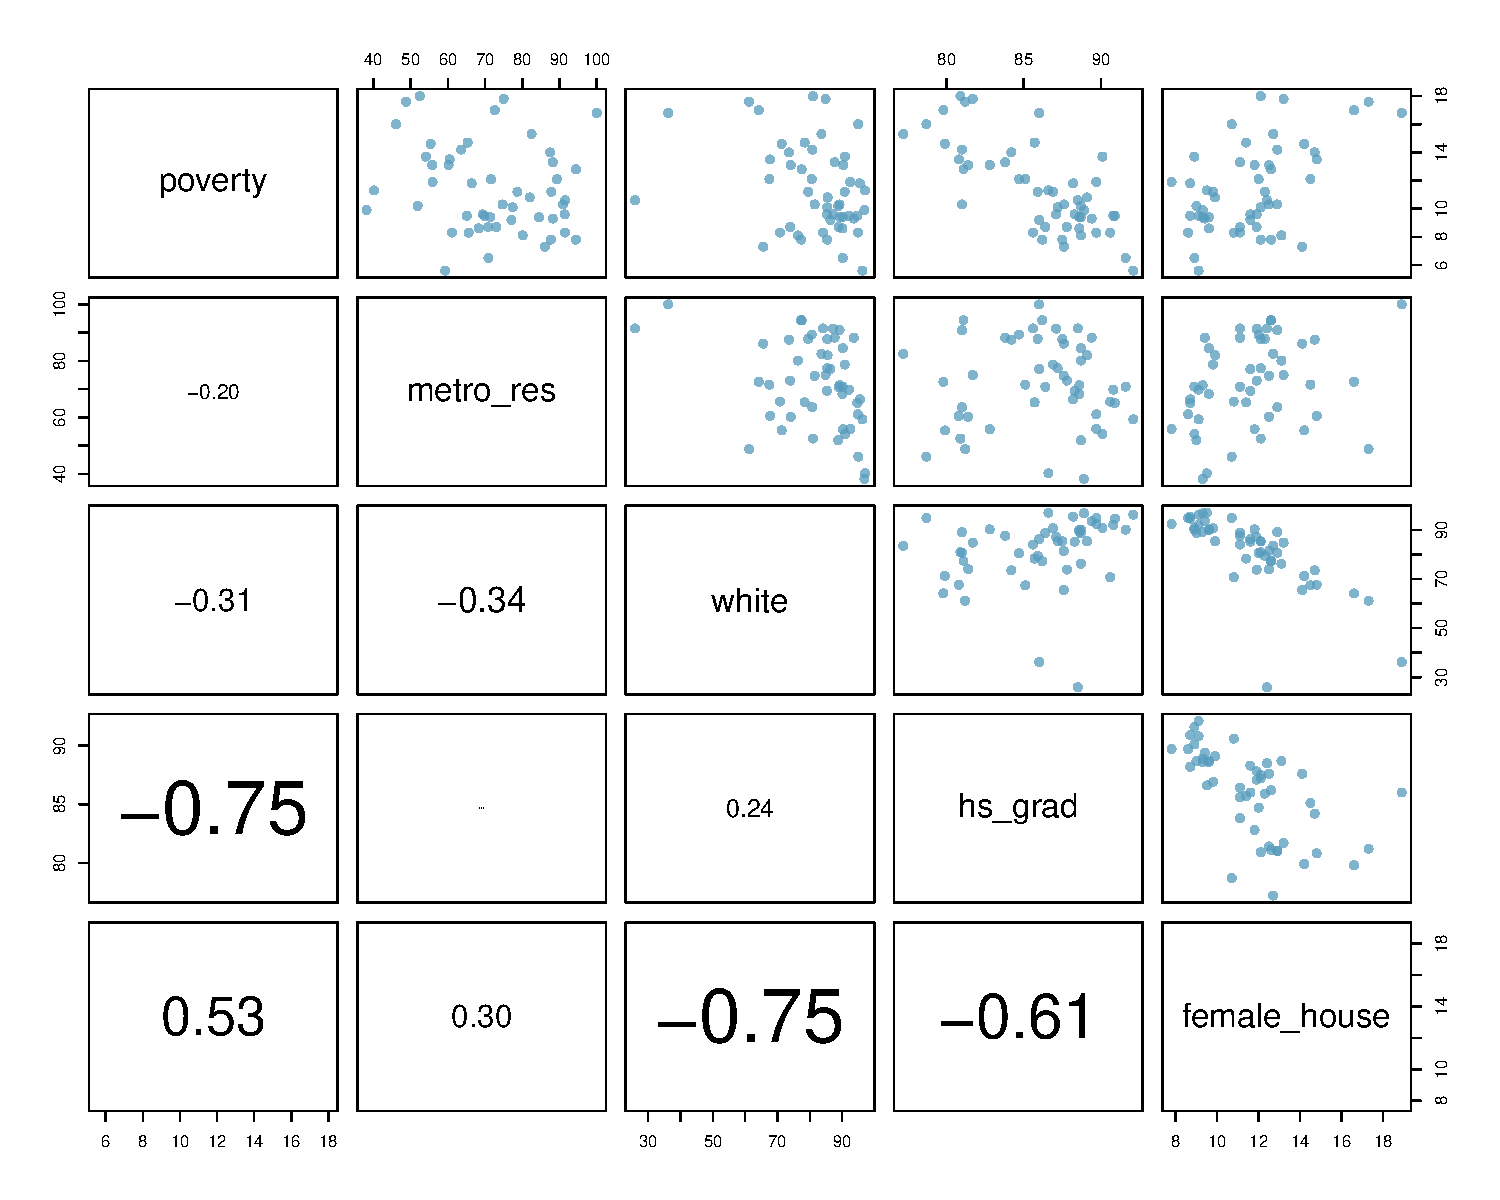
\includegraphics[width=0.8\textwidth]{9-1_intro_mlr/figures/poverty/poverty}
\end{center}

\end{frame}

%%%%%%%%%%%%%%%%%%%%%%%%%%%%%%%%%%%

\begin{frame}
\frametitle{Collinearity between explanatory variables}

\hl{poverty vs. \% female head of household}
\begin{center}
\begin{tabular}{rrrrr}
  \hline
 & Estimate & Std. Error & t value & Pr($>$$|$t$|$) \\ 
  \hline
(Intercept) & 3.31 & 1.90 & 1.74 & 0.09 \\ 
  female\_house & \only<1>{0.69} \only<2>{\orange{0.69}} & 0.16 & 4.32 & 0.00 \\ 
   \hline
\end{tabular}
\end{center}

$\:$ \\

\hl{poverty vs. \% female head of household and \% female hh}
\begin{center}
\begin{tabular}{rrrrr}
  \hline
 & Estimate & Std. Error & t value & Pr($>$$|$t$|$) \\ 
  \hline
(Intercept) & -2.58 & 5.78 & -0.45 & 0.66 \\ 
  female\_house & \only<1>{0.89} \only<2>{\orange{0.89}}  & 0.24 & 3.67 & 0.00 \\ 
  white & 0.04 & 0.04 & 1.08 & 0.29 \\   
   \hline
\end{tabular}
\end{center}

\end{frame}

%%%%%%%%%%%%%%%%%%%%%%%%%%%%%%%%%%%

\begin{frame}
\frametitle{Collinearity between explanatory variables (cont.)}

\begin{itemize}

\item Two predictor variables are said to be collinear when they are correlated, and this \hl{collinearity} complicates model estimation. \\
\Remember{Predictors are also called explanatory or \underline{independent} variables. Ideally, they would be independent of each other.}

\pause

\item We don't like adding predictors that are associated with each other to the model, because often times the addition of such variable brings nothing to the table. Instead, we prefer the simplest best model, i.e. \hl{parsimonious} model.

\pause

\item While it's impossible to avoid collinearity from arising in observational data, experiments are usually designed to prevent correlation among predictors.

\end{itemize}

\end{frame}

%%%%%%%%%%%%%%%%%%%%%%%%%%%%%%%%%%%
%
%
%\begin{frame}[fragile]
%\frametitle{F-test}
%
%ANOVA uses an F-test, which evaluates whether or not the $R^2$ is significant.
%
%
%
%\end{frame}
%
%%%%%%%%%%%%%%%%%%%%%%%%%%%%%%%%%%%%

\begin{frame}[fragile]
\frametitle{$R^2$ vs. adjusted $R^2$}

\renewcommand\arraystretch{1.25}
\begin{center}
\begin{tabular}{l | c  c}
			& $R^2$	& Adjusted $R^2$ \\
\hline
Model 1 (Single-predictor)	& 0.28	& 0.26 \\
Model 2 (Multiple)			& 0.29	& 0.26 	
\end{tabular}
\end{center}

\pause

\begin{itemize}

\item When \underline{any} variable is added to the model $R^2$ increases.

\pause

\item But if the added variable doesn't really provide any new information, or is completely unrelated, adjusted $R^2$ does not increase.

\end{itemize}



\end{frame}

%%%%%%%%%%%%%%%%%%%%%%%%%%%%%%%%%%%

\begin{frame}
\frametitle{Adjusted $R^2$}

\formula{Adjusted $R^2$}
{\[ R^2_{adj} = 1 - \pr{ \frac{ SS_{Error} }{ SS_{Total} } \times \frac{n - 1}{n - p - 1} } \]
where $n$ is the number of cases and $p$ is the number of predictors (explanatory variables) in the model.
}

\begin{itemize}

\item Because $p$ is never negative, $R^2_{adj}$ will always be smaller than $R^2$.

\item $R^2_{adj}$ applies a penalty for the number of predictors included in the model.

\item Therefore, we choose models with higher $R^2_{adj}$ over others.

\end{itemize}

\end{frame}

%%%%%%%%%%%%%%%%%%%%%%%%%%%%%%%%%%%

\begin{frame}
\frametitle{Calculate adjusted $R^2$}

\begin{center}
\begin{tabular}{lrrrrr}
  \hline
\hl{ANOVA:} & Df & Sum Sq & Mean Sq & F value & Pr($>$F) \\ 
  \hline
female\_house & 1 & 132.57 & 132.57 & 18.74 & 0.0001 \\ 
  white & 1 & 8.21 & 8.21 & 1.16 & 0.2868 \\ 
  Residuals & 48 & 339.47 & 7.07 &  &  \\ 
   \hline
Total & 50 &    480.25\\
   \hline
\end{tabular}
\end{center}

\begin{eqnarray*}
R^2_{adj} &=& 1 - \pr{ \frac{ SS_{Error} }{ SS_{Total} } \times \frac{n - 1}{n - p - 1} } \\
\pause
&=& 1 - \pr{ \frac{ 339.47 }{ 480.25 } \times \frac{51 - 1}{51 - 2 - 1} }   \\
\pause
&=& 1- \pr{ \frac{ 339.47 }{ 480.25 } \times \frac{50}{48} } \\
\pause
&=& 1 -  0.74 \\
\pause
&=& 0.26
\end{eqnarray*}

\end{frame}

%%%%%%%%%%%%%%%%%%%%%%%%%%%%%%%%%%%%

\section{Model selection}

%%%%%%%%%%%%%%%%%%%%%%%%%%%%%%%%%%%%

\subsection{Identifying variables in the model that may not be helpful}

%%%%%%%%%%%%%%%%%%%%%%%%%%%%%%%%%%%

\begin{frame}
\frametitle{Beauty in the classroom}

\begin{itemize}

\item Data: Student evaluations of instructors' beauty and teaching quality for 463 courses at the University of Texas.

\item Evaluations conducted at the end of semester, and the beauty judgements were made later, by six students who had not attended the classes and were not aware of the course evaluations (2 upper level females, 2 upper level males, one lower level female, one lower level male).

\end{itemize}

\ct{Hamermesh \& Parker. (2004)``Beauty in the classroom: instructors? pulchritude and putative pedagogical productivity? Economics Education Review.}

\end{frame}

%%%%%%%%%%%%%%%%%%%%%%%%%%%%%%%%%%%

\begin{frame}
\frametitle{Professor rating vs. beauty}

Professor evaluation score (higher score means better) vs. beauty score (a score of 0 means average, negative score means below average, and a positive score above average):

\begin{center}
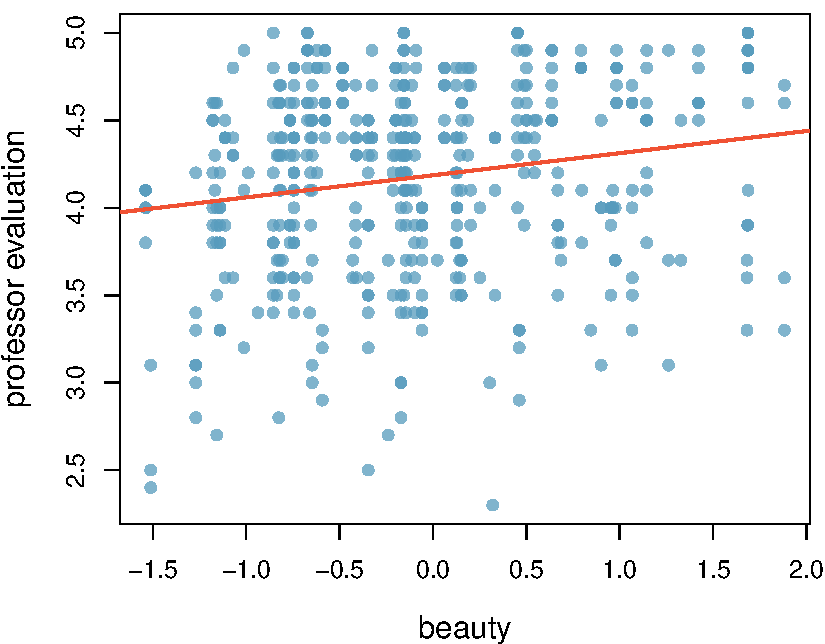
\includegraphics[width=0.65\textwidth]{9-2_model_select/figures/beauty/beauty_profeval}
\end{center}

\end{frame}

%%%%%%%%%%%%%%%%%%%%%%%%%%%%%%%%%%%

\begin{frame}
\frametitle{}

\pq{Which of the below is \underline{correct} based on the model output?}

\begin{center}
{\small
\begin{tabular}{rrrrr}
  \hline
 & Estimate & Std. Error & t value & Pr($>$$|$t$|$) \\ 
  \hline
(Intercept) & 4.19 & 0.03 & 167.24 & 0.00 \\ 
  beauty & 0.13 & 0.03 & 4.00 & 0.00 \\
   \hline
$R^2$ = 0.0336
\end{tabular}
}
\end{center}

\begin{enumerate}[(a)]
\item Model predicts 3.36\% of professor ratings correctly.
\item Beauty is not a significant predictor of professor evaluation.
\solnMult{Professors who score 1 point above average in their beauty score are tend to also score 0.13 points higher in their evaluation.}
\item 3.36\% of variability in beauty scores can be explained by professor evaluation.
\item The correlation coefficient could be $\sqrt{0.0336} = 0.18$ or $-0.18$, we can't tell which is correct.
\end{enumerate}

\end{frame}

%%%%%%%%%%%%%%%%%%%%%%%%%%%%%%%%%%%

\begin{frame}
\frametitle{Exploratory analysis}

\twocol{0.4}{0.6}
{
\dq{Any interesting features?}
\soln{\only<2->{Few females with very low beauty scores.}}
$\:$ \\
\dq{For a given beauty score, are male professors evaluated higher, lower, or about the same as female professors?}
\soln{\only<3->{Difficult to tell from this plot only.}}
}
{
\begin{center}
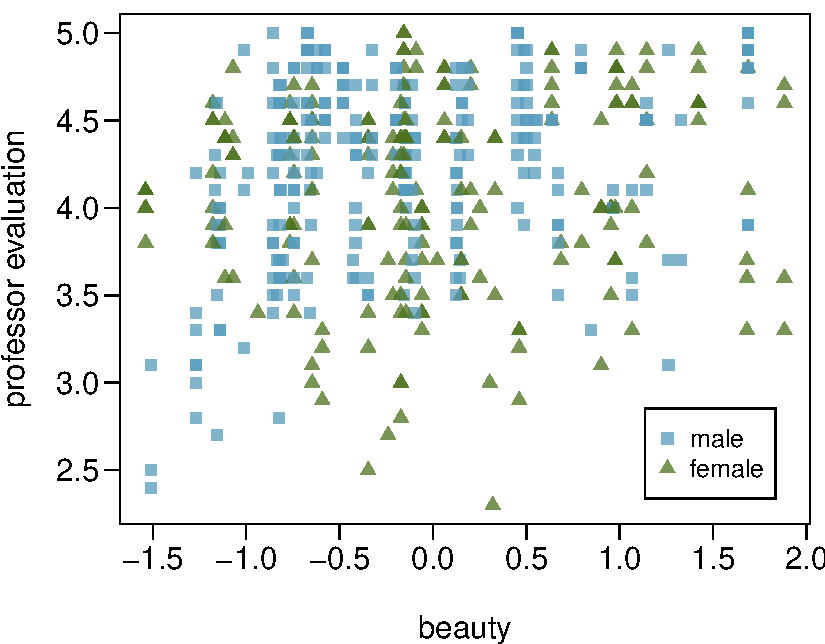
\includegraphics[width=\textwidth]{9-2_model_select/figures/beauty/beauty_profeval_gender}
\end{center}
}

\end{frame}

%%%%%%%%%%%%%%%%%%%%%%%%%%%%%%%%%%

\begin{frame}[fragile]
\frametitle{Professor rating vs. beauty + gender}

\pq{For a given beauty score, are male professors evaluated higher, lower, or about the same as female professors?}

{\small
\begin{center}
\begin{tabular}{rrrrr}
  \hline
 & Estimate & Std. Error & t value & Pr($>$$|$t$|$) \\ 
  \hline
(Intercept) & 4.09 & 0.04 & 107.85 & 0.00 \\ 
  beauty & 0.14 & 0.03 & 4.44 & 0.00 \\ 
  gender.male & 0.17 & 0.05 & 3.38 & 0.00 \\ 
   \hline
$R^2_{adj}$ = 0.057
\end{tabular}
\end{center}
}

\begin{enumerate}[(a)]
\solnMult{higher} \soln{\only<2>{\orange{$\rightarrow$ Beauty held constant, male professors are rated 0.17 points higher on average than female professors.}}}
\item lower
\item about the same
\end{enumerate}

\end{frame}

%%%%%%%%%%%%%%%%%%%%%%%%%%%%%%%%%%%

\begin{frame}[fragile]
\frametitle{Full model}

{\small
\begin{center}
\begin{tabular}{rrrrr}
  \hline
 & Estimate & Std. Error & t value & Pr($>$$|$t$|$) \\ 
  \hline
(Intercept) & 4.6282 & 0.1720 & 26.90 & 0.00 \\ 
  beauty & 0.1080 & 0.0329 & 3.28 & 0.00 \\ 
  gender.male & 0.2040 & 0.0528 & 3.87 & 0.00 \\ 
  age & -0.0089 & 0.0032 & -2.75 & 0.01 \\ 
formal.yes \footnote{\texttt{formal}: picture wearing tie\&jacket/blouse, levels: \texttt{yes}, \texttt{no}} & 0.1511 & 0.0749 & 2.02 & 0.04 \\ 
  lower.yes \footnote{\texttt{lower}: lower division course, levels: \texttt{yes}, \texttt{no}} & 0.0582 & 0.0553 & 1.05 & 0.29 \\ 
  native.non english & -0.2158 & 0.1147 & -1.88 & 0.06 \\ 
  minority.yes & -0.0707 & 0.0763 & -0.93 & 0.35 \\ 
  students \footnote{\texttt{students}: number of students} & -0.0004 & 0.0004 & -1.03 & 0.30 \\ 
  tenure.tenure track \footnote{\texttt{tenure}: tenure status, levels: \texttt{non-tenure track}, \texttt{tenure track}, \texttt{tenured}} & -0.1933 & 0.0847 & -2.28 & 0.02 \\ 
  tenure.tenured & -0.1574 & 0.0656 & -2.40 & 0.02 \\ 
   \hline
\end{tabular}
\end{center}
}

\end{frame}

%%%%%%%%%%%%%%%%%%%%%%%%%%%%%%%%%%%

\begin{frame}
\frametitle{Hypotheses}

Just as the interpretation of the slope parameters take into account all other variables in the model,  the hypotheses for testing for significance of a predictor also takes into account all other variables.

$\:$ \\

\begin{itemize}
\item[] \mathhl{H_0:} $B_i = 0$ when other explanatory variables are included in the model.
\item[] \mathhl{H_A:} $B_i \ne 0$ when other explanatory variables are included in the model.
\end{itemize}

\end{frame}

%%%%%%%%%%%%%%%%%%%%%%%%%%%%%%%%%%%

\begin{frame}
\frametitle{Assessing significance: numerical variables}

\pq{The p-value for age is 0.01. What does this indicate?}

{\scriptsize
\begin{center}
\begin{tabular}{rrrrr}
  \hline
 & Estimate & Std. Error & t value & Pr($>$$|$t$|$) \\ 
  \hline
...\\
  age & -0.0089 & 0.0032 & -2.75 & 0.01 \\ 
...\\
   \hline
\end{tabular}
\end{center}
}

\begin{enumerate}[(a)]
\item Since p-value is positive, higher the professor's age, the higher we would expect them to be rated.
\solnMult{If we keep all other variables in the model, there is strong evidence that professor's age is associated with their rating.}
\item Probability that the true slope parameter for age is 0 is 0.01.
\item There is about 1\% chance that the true slope parameter for age is -0.0089.
\end{enumerate}

\end{frame}

%%%%%%%%%%%%%%%%%%%%%%%%%%%%%%%%%%%

\begin{frame}[fragile]
\frametitle{Assessing significance: categorical variables}

\pq{{\small Tenure is a categorical variable with 3 levels: non tenure track, tenure track, tenured. Based on the model output given, which of the below is \underline{false}?}}

{\footnotesize
\begin{center}
\begin{tabular}{rrrrr}
  \hline
 & Estimate & Std. Error & t value & Pr($>$$|$t$|$) \\ 
  \hline
... \\
  tenure.tenure track & -0.1933 & 0.0847 & -2.28 & 0.02 \\ 
  tenure.tenured & -0.1574 & 0.0656 & -2.40 & 0.02 \\ 
   \hline
\end{tabular}
\end{center}
}

\begin{enumerate}[(a)]
\item Reference level is non tenure track.
\item All else being equal, tenure track professors are rated, on average, 0.19 points lower than non-tenure track professors.
\item All else being equal, tenured professors are rated, on average, 0.16 points lower than non-tenure track professors.
\solnMult{All else being equal, there is a significant difference between the average ratings of tenure track and tenured professors.}
\end{enumerate}

\end{frame}

%%%%%%%%%%%%%%%%%%%%%%%%%%%%%%%%%%%

\begin{frame}
\frametitle{Assessing significance}

\dq{Which predictors do not seem to meaningfully contribute to the model, i.e. may not be significant predictors of professor's rating score?}

{\scriptsize
\begin{center}
\begin{tabular}{rrrrr}
  \hline
 & Estimate & Std. Error & t value & Pr($>$$|$t$|$) \\ 
  \hline
(Intercept) & 4.6282 & 0.1720 & 26.90 & 0.00 \\ 
  beauty & 0.1080 & 0.0329 & 3.28 & 0.00 \\ 
  gender.male & 0.2040 & 0.0528 & 3.87 & 0.00 \\ 
  age & -0.0089 & 0.0032 & -2.75 & 0.01 \\ 
  formal.yes & 0.1511 & 0.0749 & 2.02 & 0.04 \\ 
  \rowcolor{oiB!50}
  lower.yes & 0.0582 & 0.0553 & 1.05 & 0.29 \\ 
    \rowcolor{oiB!50}
  native.non english & -0.2158 & 0.1147 & -1.88 & 0.06 \\ 
    \rowcolor{oiB!50}
  minority.yes & -0.0707 & 0.0763 & -0.93 & 0.35 \\ 
    \rowcolor{oiB!50}
  students & -0.0004 & 0.0004 & -1.03 & 0.30 \\ 
  tenure.tenure track & -0.1933 & 0.0847 & -2.28 & 0.02 \\ 
  tenure.tenured & -0.1574 & 0.0656 & -2.40 & 0.02 \\ 
   \hline
\end{tabular}
\end{center}
}

\end{frame}

%%%%%%%%%%%%%%%%%%%%%%%%%%%%%%%%%%%

\subsection{Two model selection strategies}

%%%%%%%%%%%%%%%%%%%%%%%%%%%%%%%%%%%

\begin{frame}
\frametitle{Model selection strategies}

\dq{Based on what we've learned so far, what are some ways you can think of that can be used to determine which variables to keep in the model and which to leave out?}

\end{frame}


%%%%%%%%%%%%%%%%%%%%%%%%%%%%%%%%%%%

\begin{frame}
\frametitle{Backward-elimination}

\begin{enumerate}

\item Start with the full model
\item Drop one variable at a time and record $R^2_{adj}$ of each smaller model
\item Pick the model with the highest increase in $R^2_{adj}$
\item Repeat until none of the models yield an increase in $R^2_{adj}$

\end{enumerate}

\end{frame}

%%%%%%%%%%%%%%%%%%%%%%%%%%%%%%%%%%%

\begin{frame}[shrink]
\frametitle{Backward-elimination}

\vspace{-0.3cm}

{\tiny
\begin{tabular}{l | l | c}
Full		& beauty + gender + age + formal + lower + native + minority + students + tenure & \orange{0.0839} \pause \\
\hline
Step 1 	& gender + age + formal + lower + native + minority + students + tenure		& 0.0642 \\
		& beauty + age + formal + lower + native + minority + students + tenure		& 0.0557 \\
		& beauty + gender + formal + lower + native + minority + students + tenure	& 0.0706 \\
		& beauty + gender + age + lower + native + minority + students + tenure		& 0.0777 \\
		& beauty + gender + age + formal + native + minority + students + tenure		& 0.0837 \\
		& beauty + gender + age + formal + lower + minority + students + tenure		& 0.0788 \\
		& beauty + gender + age + formal + lower + native + students + tenure		& \orange{0.0842} \\
		& beauty + gender + age + formal + lower + native + minority + tenure		& 0.0838 \\
		& beauty + gender + age + formal + lower + native + minority + students		& 0.0733 \pause \\
\hline		
Step 2	& gender + age + formal + lower + native + students + tenure 				& 0.0647 \\
		& beauty + age + formal + lower + native + students + tenure 				& 0.0543 \\
		& beauty + gender + formal + lower + native + students + tenure 			& 0.0708 \\
		& beauty + gender + age + lower + native + students + tenure 				&0.0776  \\
		& beauty + gender + age + formal + native + students + tenure 			& \orange{0.0846} \\
		& beauty + gender + age + formal + lower + native + tenure 				& 0.0844 \\
		& beauty + gender + age + formal + lower + native + students 				& 0.0725 \pause \\
\hline
Step 3	& gender + age + formal + native + students + tenure 					& 0.0653 \\
		& beauty + age + formal + native + students + tenure					& 0.0534 \\
		& beauty + gender + formal + native + students + tenure					& 0.0707 \\
		& beauty + gender + age + native + students + tenure					& 0.0786 \\
		& beauty + gender + age + formal + students + tenure					& 0.0756 \\
		& beauty + gender + age + formal + native + tenure						& \orange{0.0855} \\
		& beauty + gender + age + formal + native + students					& 0.0713 \pause \\
\hline
Step 4	& gender + age + formal + native + tenure 							& 0.0667 \\
		& beauty + age + formal + native + tenure								& 0.0553 \\
		& beauty + gender + formal + native + tenure							& 0.0723 \\
		& beauty + gender + age + native + tenure							& 0.0806 \\
		& beauty + gender + age + formal + tenure							& 0.0773 \\
		& beauty + gender + age + formal + native							& 0.0713 \\
\end{tabular}
}

\end{frame}

%%%%%%%%%%%%%%%%%%%%%%%%%%%%%%%%%%%

\begin{frame}[fragile]
\frametitle{\texttt{step} function in R}

The \texttt{step} function in R does a similar backward elimination process, 
however it uses a different metric called AIC (Akaike Information Criterion) 
instead of adjusted $R^2$ to do the model selection.

{\tiny
\begin{verbatim}
Call:
lm(formula = profevaluation ~ beauty + gender + age + formal + 
    native + tenure, data = d)

Coefficients:
       (Intercept)              beauty          gendermale  
          4.628435            0.105546            0.208079  
               age           formalyes   nativenon english  
         -0.008844            0.132422           -0.243003  
tenuretenure track       tenuretenured  
         -0.206784           -0.175967  
\end{verbatim}
}

\pause
Best model: beauty + gender + age + formal + native + tenure

\end{frame}

%%%%%%%%%%%%%%%%%%%%%%%%%%%%%%%%%%%

\begin{frame}
\frametitle{Forward selection}

\begin{enumerate}

\item Start with regressions of response vs. each explanatory variable
\item Pick the model with the highest $R^2_{adj}$
\item Add the remaining variables one at a time to the existing model, and once again pick the model  with the highest $R^2_{adj}$
\item Repeat until the addition of any of the remanning variables does not result in a higher $R^2_{adj}$

\end{enumerate}

\end{frame}

%%%%%%%%%%%%%%%%%%%%%%%%%%%%%%%%%%%

\subsection{The p-value approach, an alternative to adjusted $R^2$}

%%%%%%%%%%%%%%%%%%%%%%%%%%%%%%%%%%%

\begin{frame}
\subsection{Backward and forward}

\begin{itemize}

\item Backward elimination with the p-value approach: 
\begin{enumerate}
\item Start with the full model
\item Drop the variable with the highest p-value and refit a smaller model
\item Repeat until all variables left in the model are significant
\end{enumerate}

\item Forward selection with the p-value approach: 
\begin{enumerate}
\item Start with regressions of response vs. each explanatory variable
\item Pick the variable with the lowest significant p-value 
\item Add the remaining variables one at a time to the existing model, and pick the variable with the lowest significant p-value
\item Repeat until any of the remaining variables does not have a significant p-value
\end{enumerate}

\end{itemize}

\end{frame}

%%%%%%%%%%%%%%%%%%%%%%%%%%%%%%%%%%%

\begin{frame}
\frametitle{Backward-elimination: $p-value$ approach}

\resizebox{\textwidth}{!}{%
{\tiny
\begin{tabular}{l | rrrrrrrrrr }
\textbf{Step}		& \multicolumn{10}{c}{ \textbf{Variables included \& p-value} } \\
\hline
Full		& beauty	& gender		& age	& formal		& lower 	& native	 	& minority		& students	& tenure		& tenure \\
		& 		& male		& 		& yes		& yes	 & nonenglish	& yes		& 			& tenure track	& tenured \\
		&  0.00 	&  0.00 		& 0.01	& 0.04		& 0.29	& 0.06		& \orange{0.35}	& 0.30		& 0.02		& 0.02 \pause \\
\hline
Step 1	& beauty	& gender		& age	& formal		& lower 		& native	 	& 			& students	& tenure		& tenure \\
		& 		& male		& 		& yes		& yes		& nonenglish	& 			& 			& tenure track	& tenured \\
		&  0.00 	&  0.00 		& 0.01	& 0.04		& \orange{0.38}	& 0.03		&			& 0.34		& 0.02		& 0.01 \pause\\
\hline
Step 2	& beauty	& gender		& age	& formal		& 	 		& native	 	& 			& students	& tenure		& tenure \\
		& 		& male		& 		& yes		& 			& nonenglish	& 			& 			& tenure track	& tenured \\
		&  0.00 	&  0.00 		& 0.01	& 0.05		& 			& 0.02		&			& \orange{0.44}	& 0.01		& 0.01\pause \\
\hline
Step 3 	& beauty	& gender		& age	& formal		& 	 		& native	 	& 			& 			& tenure		& tenure \\
		& 		& male		& 		& yes		& 			& nonenglish	& 			& 			& tenure track	& tenured \\
		&  0.00 	&  0.00 		& 0.01	& \orange{0.06}	& 			& 0.02		&			& 			& 0.01		& 0.01 \pause \\
\hline
Step 	4	& beauty	& gender		& age	& 			& 	 		& native	 	& 			& 			& tenure		& tenure \\
		& 		& male		& 		& 			& 			& nonenglish	& 			& 			& tenure track	& tenured \\
		&  0.00 	&  0.00 		& 0.01	&			& 			& \orange{0.06}	&			& 			& 0.01		& 0.01 \pause \\
\hline
Step 5 	& beauty	& gender		& age	& 			& 	 		& 		 	& 			& 			& tenure		& tenure \\
		& 		& male		& 		& 			& 			&			& 			& 			& tenure track	& tenured \\
		&  0.00 	&  0.00 		& 0.01	&			& 			& 			&			& 			& 0.01		& 0.01 \\
\end{tabular}
}}

$\:$ \\

\pause
Best model: beauty + gender + age + tenure

\end{frame}

%%%%%%%%%%%%%%%%%%%%%%%%%%%%%%%%%%%

\begin{frame}
\frametitle{Adjusted $R^2$ vs. p-value approaches}

\begin{itemize}

\item The two approaches are similar, but they sometimes lead to different models, with the adjusted $R^2$ approach tending to include more predictors in the final model.

\item When the sole goal is to improve prediction accuracy, use $R^2$ . This is commonly the case in machine learning applications.

\item When we care about understanding which variables are statistically significant predictors of the response, or if there is interest in producing a simpler model at the potential cost of a little prediction accuracy, then the p-value approach is preferred.

\item Regardless of the approach we use, our job is not done after variable selection -- we must still verify the model conditions are reasonable.

\end{itemize}

\end{frame}

%%%%%%%%%%%%%%%%%%%%%%%%%%%%%%%%%%%

%%%%%%%%%%%%%%%%%%%%%%%%%%%%%%%%%%%%

\section{Checking model conditions using graphs}

%%%%%%%%%%%%%%%%%%%%%%%%%%%%%%%%%%%%

\begin{frame}
\frametitle{Modeling conditions}

\[ \hat{y} = \beta_0 + \beta_1 x_1 + \beta_2 x_2 + \cdots + \beta_p x_p \] 

$\:$ \\

The model depends on the following conditions
\begin{enumerate}
\item residuals are nearly normal (primary concern relates to residuals that are outliers)
\item residuals have constant variability
\item residuals are independent
\item each variable is linearly related to the outcome \\
\end{enumerate}

We often use graphical methods to check the validity of these conditions, which we will go through in detail in the following slides.

\end{frame}

%%%%%%%%%%%%%%%%%%%%%%%%%%%%%%%%%%

\begin{frame}
\frametitle{(1) nearly normal residuals}

normal probability plot and/or histogram of residuals: \\

\begin{center}
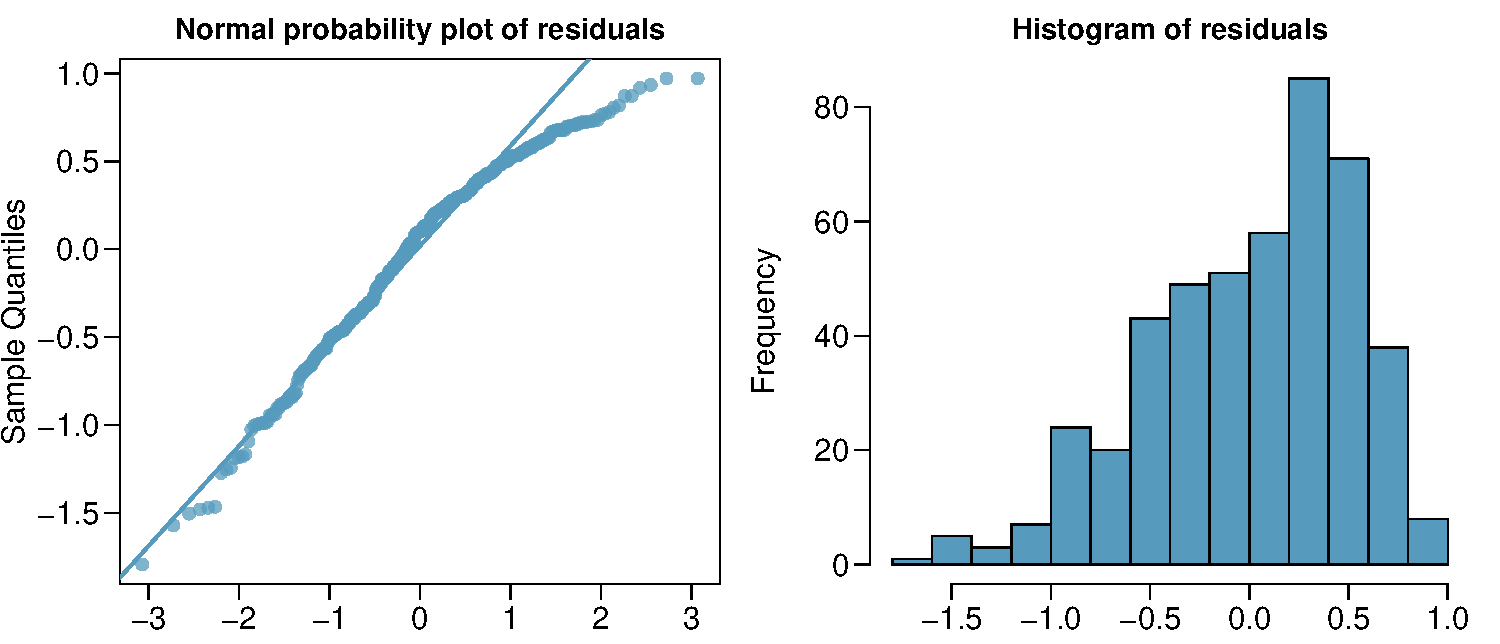
\includegraphics[width=\textwidth]{9-3_model_cond/figures/beauty/normal_res}
\end{center}

\dq{Does this condition appear to be satisfied?}

\end{frame}

%%%%%%%%%%%%%%%%%%%%%%%%%%%%%%%%%%

\begin{frame}
\frametitle{(2) constant variability in residuals}

scatterplot of residuals and/or absolute value of residuals vs. fitted (predicted): \\

\begin{center}
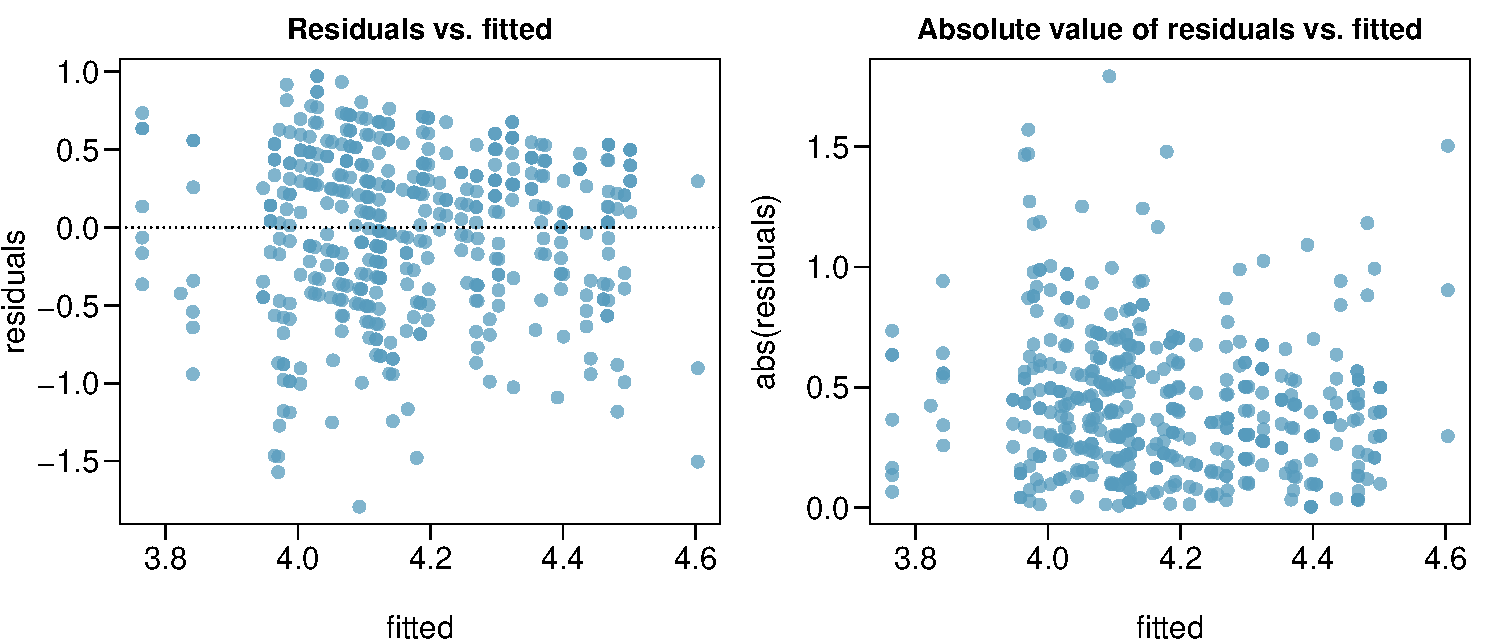
\includegraphics[width=\textwidth]{9-3_model_cond/figures/beauty/homo_res}
\end{center}

\dq{Does this condition appear to be satisfied?}

\end{frame}

%%%%%%%%%%%%%%%%%%%%%%%%%%%%%%%%%%

\begin{frame}
\frametitle{Checking constant variance - recap}

\begin{itemize}

\item When we did simple linear regression (one explanatory variable) we checked the constant variance condition using a plot of \hl{residuals vs. x}.

\item With multiple linear regression (2+ explanatory variables) we checked the constant variance condition using a plot of \hl{residuals vs. fitted}. 

\end{itemize}

$\:$ \\

\dq{Why are we using different plots?}

\soln{\only<2>{In multiple linear regression there are many explanatory variables, so a plot of residuals vs. one of them wouldn't give us the complete picture.
}}

\end{frame}

%%%%%%%%%%%%%%%%%%%%%%%%%%%%%%%%%%

\begin{frame}[fragile]
\frametitle{(3) independent residuals}

scatterplot of residuals vs. order of data collection: \\

\begin{center}
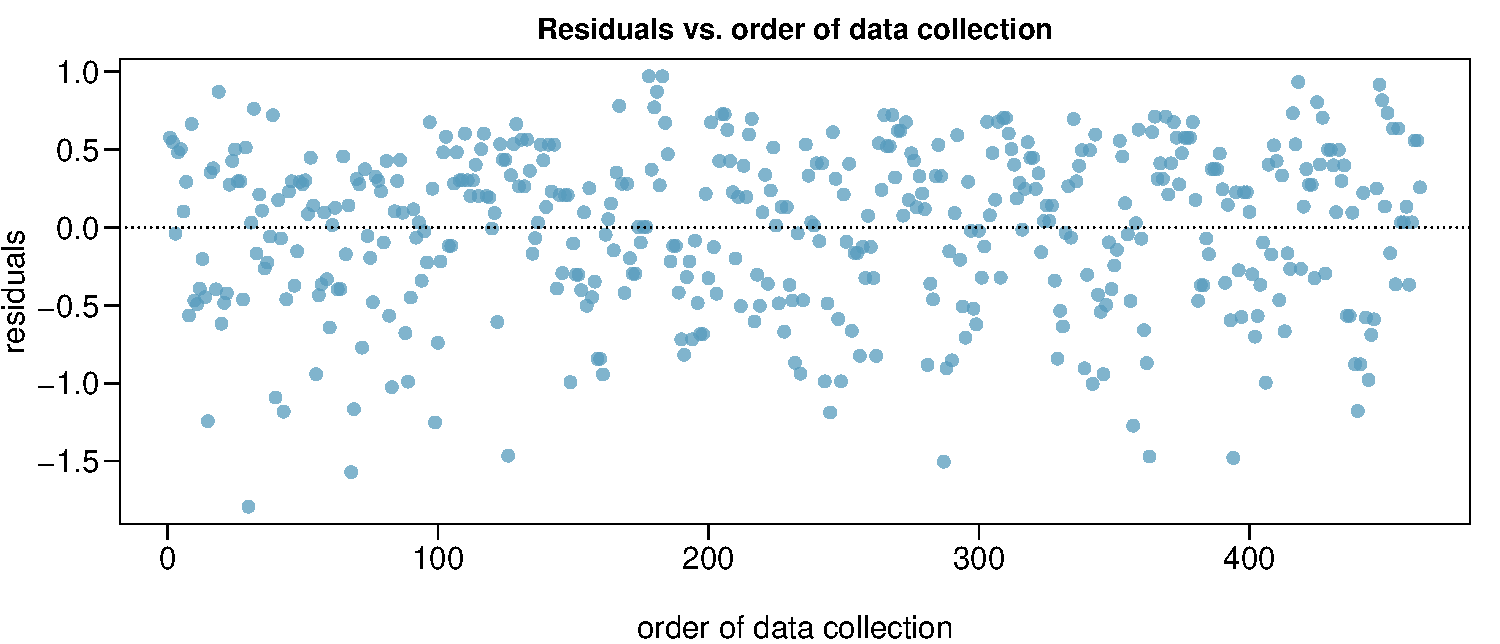
\includegraphics[width=0.8\textwidth]{9-3_model_cond/figures/beauty/indep_res}
\end{center}

\dq{Does this condition appear to be satisfied?}

\end{frame}

%%%%%%%%%%%%%%%%%%%%%%%%%%%%%%%%%%

\begin{frame}
\frametitle{More on the condition of independent residuals}

\begin{itemize}

\item Checking for independent residuals allows us to indirectly check for independent observations.

\item If observations and residuals are independent, we would not expect to see an increasing or decreasing trend in the scatterplot of residuals vs. order of data collection.

\item This condition is often violated when we have time series data. Such data require more advanced time series regression techniques for proper analysis.

\end{itemize}

\end{frame}

%%%%%%%%%%%%%%%%%%%%%%%%%%%%%%%%%%

\begin{frame}[fragile]
\frametitle{(4) linear relationships}

scatterplot of residuals vs. each (numerical) explanatory variable:

\begin{center}
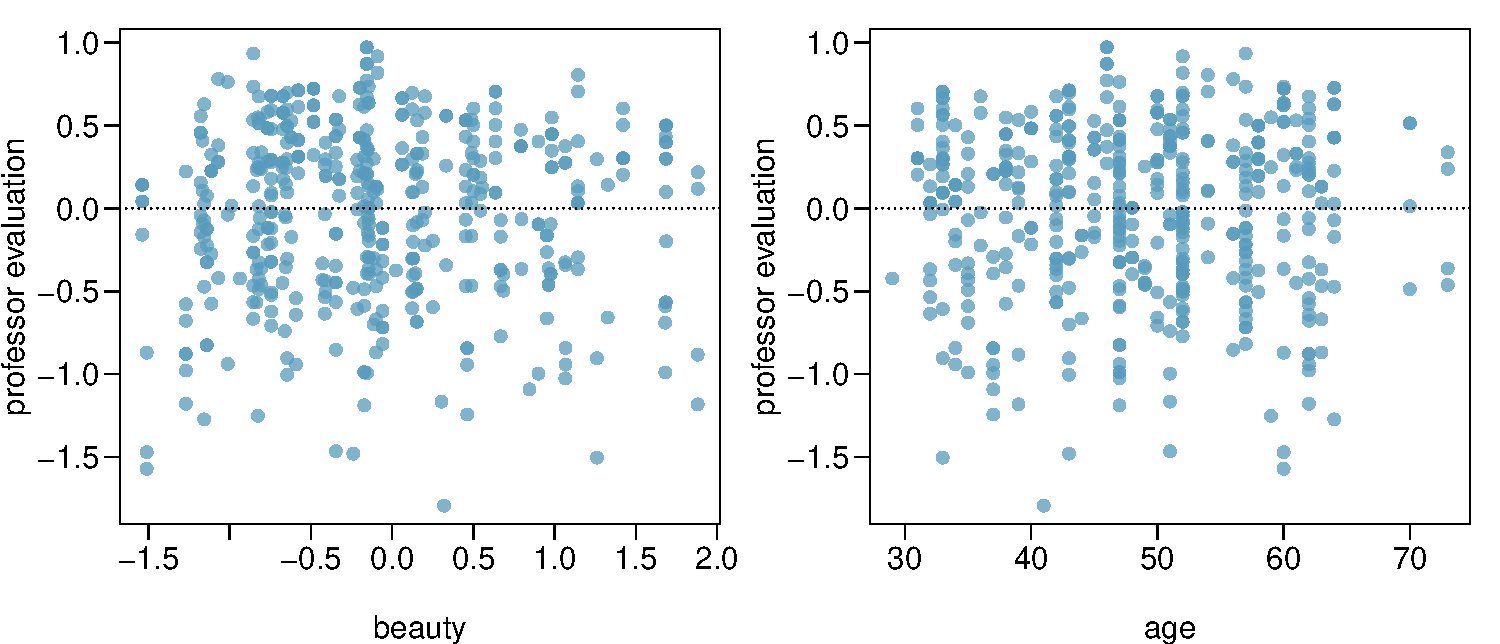
\includegraphics[width=0.8\textwidth]{9-3_model_cond/figures/beauty/linear}
\end{center}

\dq{Does this condition appear to be satisfied?}

\Note{We use residuals instead of the predictors on the y-axis so that we can still check for linearity without worrying about other possible violations like collinearity between the predictors.}

\end{frame}

%%%%%%%%%%%%%%%%%%%%%%%%%%%%%%%%%%%
%\input{9-4_mlr_case_study/9-4_mlr_case_study}
%%%%%%%%%%%%%%%%%%%%%%%%%%%%%%%%%%%%

\section{Logistic regression}

%%%%%%%%%%%%%%%%%%%%%%%%%%%%%%%%%%%%

\begin{frame}
\frametitle{Regression so far ...}
    
At this point we have covered:

{\small
\begin{itemize}
\item Simple linear regression
\begin{itemize}
\item Relationship between numerical response and a numerical or categorical predictor
\end{itemize}
\pause
\item Multiple regression
\begin{itemize}
\item Relationship between numerical response and multiple numerical and/or categorical predictors
\end{itemize}
\end{itemize}
}

\pause

What we haven't seen is what to do when the predictors are weird (nonlinear, complicated dependence structure, etc.) or when the response is weird (categorical, count data, etc.)


\end{frame}

%%%%%%%%%%%%%%%%%%%%%%%%%%%%%%%%%%%

\begin{frame}
\frametitle{Odds}

\vspace{-2mm}

Odds are another way of quantifying the probability of an event, commonly used in gambling (and logistic regression).\\

~\\

\formula{Odds}
{
For some event $E$,
{\small
\[\text{odds}(E) = \frac{P(E)}{P(E^c)} = \frac{P(E)}{1-P(E)}\]
}
Similarly, if we are told the odds of E are $x$ to $y$ then
{\small
\[\text{odds}(E) = \frac{x}{y} = \frac{x/(x+y)}{y/(x+y)} \]
}
which implies
{\small
\[P(E) = x/(x+y),\quad P(E^c) = y/(x+y)\]
}
}

\end{frame}

%%%%%%%%%%%%%%%%%%%%%%%%%%%%%%%%%%%

\subsection{Generalized linear models}

%%%%%%%%%%%%%%%%%%%%%%%%%%%%%%%%%%%

\begin{frame}
\frametitle{Example - Donner Party}

In 1846 the Donner and Reed families left Springfield, Illinois, for California by covered wagon. In July, the Donner Party, as it became known, reached Fort Bridger, Wyoming. There its leaders decided to attempt a new and untested rote to the Sacramento Valley. Having reached its full size of 87 people and 20 wagons, the party was delayed by a difficult crossing of the Wasatch Range and again in the crossing of the desert west of the Great Salt Lake. The group became stranded in the eastern Sierra Nevada mountains when the region was hit by heavy snows in late October. By the time the last survivor was rescued on April 21, 1847, 40 of the 87 members had died from famine and exposure to extreme cold.\\


\vfill

{\tiny From \textit{Ramsey, F.L. and Schafer, D.W. (2002). The Statistical Sleuth: A Course in Methods of Data Analysis (2nd ed)}}
\end{frame}


%%%%%%%%%%%%%%%%%%%%%%%%%%%%%%%%%%%

\begin{frame}
\frametitle{Example - Donner Party - Data}

\begin{center}
\begin{tabular}{rlll}
  \hline
     & Age   & Sex    & Status \\ 
  \hline
   1 & 23.00 & Male   & Died \\ 
   2 & 40.00 & Female & Survived \\ 
   3 & 40.00 & Male   & Survived \\ 
   4 & 30.00 & Male   & Died \\ 
   5 & 28.00 & Male   & Died \\ 
\vdots & ~~~\vdots & ~~~\vdots & ~~~\vdots \\
  43 & 23.00 & Male   & Survived \\ 
  44 & 24.00 & Male   & Died \\ 
  45 & 25.00 & Female & Survived \\ 
   \hline
\end{tabular}
\end{center}

\end{frame}

%%%%%%%%%%%%%%%%%%%%%%%%%%%%%%%%%%%
\begin{frame}
\frametitle{Example - Donner Party - EDA}

Status vs. Gender:\\

\begin{center}
\begin{tabular}{rrr}
\hline
         & Male & Female \\ 
\hline
Died     &  20  &   5 \\ 
Survived &  10  &  10 \\ 
   \hline
\end{tabular}
\end{center}

\pause 
\vfill

Status vs. Age:\\
\begin{center}
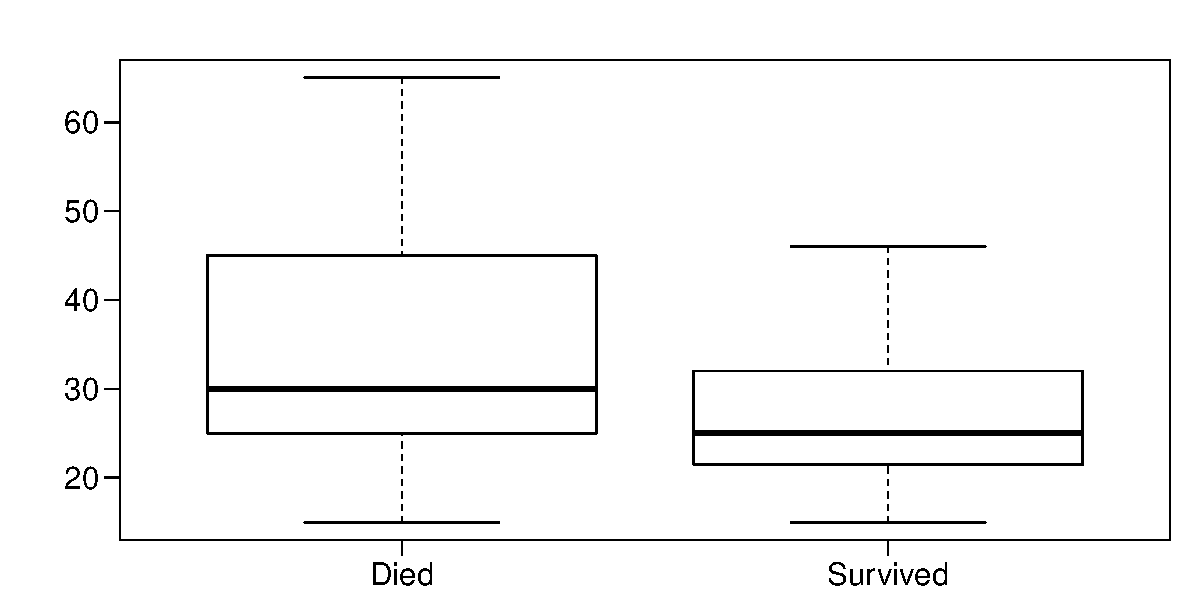
\includegraphics[width=0.8\textwidth]{9-5_logistic_reg/figures/donner/status_age}
\end{center}

\end{frame}

%%%%%%%%%%%%%%%%%%%%%%%%%%%%%%%%%%%

\begin{frame}
\frametitle{Example - Donner Party}

It seems clear that both age and gender have an effect on someone's survival, how do we come up with a model that will let us explore this relationship?\\

~\\ \pause

Even if we set Died to 0 and Survived to 1, this isn't something we can transform our way out of - we need something more.

~\\ \pause

One way to think about the problem - we can treat Survived and Died as successes and failures arising from a binomial distribution where the probability of a success is given by a transformation of a linear model of the predictors.

\end{frame}

%%%%%%%%%%%%%%%%%%%%%%%%%%%%%%%%%%%

\begin{frame}
\frametitle{Generalized linear models}

It turns out that this is a very general way of addressing this type of problem in regression, and the resulting models are called generalized linear models (GLMs). Logistic regression is just one example of this type of model.\\
~\\
\pause
All generalized linear models have the following three characteristics:
\begin{enumerate}
\item A probability distribution describing the outcome variable 
\item A linear model
\begin{itemize}
\item $\eta = \beta_0+\beta_1 X_1 + \cdots + \beta_n X_n$
\end{itemize}
\item A link function that relates the linear model to the parameter of the outcome distribution
\begin{itemize}
\item $g(p) = \eta$ or $p = g^{-1}(\eta)$
\end{itemize}
\end{enumerate}

\end{frame}

%%%%%%%%%%%%%%%%%%%%%%%%%%%%%%%%%%%

\subsection{Logistic Regression}

%%%%%%%%%%%%%%%%%%%%%%%%%%%%%%%%%%%

\begin{frame}
\frametitle{Logistic Regression}

Logistic regression is a GLM used to model a binary categorical variable using numerical and categorical predictors.\\
~\\
We assume a binomial distribution produced the outcome variable and we therefore want to model $p$ the probability of success for a given set of predictors.\\
~\\

\pause

To finish specifying the Logistic model we just need to establish a reasonable link function that connects $\eta$ to $p$. There are a variety of options but the most commonly used is the logit function.\\

~\\

\formula{Logit function}{
\[logit(p) = \log\left(\frac{p}{1-p}\right),\text{ for $0\le p \le 1$}\]
}

\end{frame}

%%%%%%%%%%%%%%%%%%%%%%%%%%%%%%%%%%%

\begin{frame}
\frametitle{Properties of the Logit}

The logit function takes a value between 0 and 1 and maps it to a value between $-\infty$ and $\infty$.\\
~\\

\formula{Inverse logit (logistic) function}
{
\[g^{-1}(x) = \frac{\exp(x)}{1+\exp(x)} = \frac{1}{1+\exp(-x)}\]
}

~\\
The inverse logit function takes a value between $-\infty$ and $\infty$ and maps it to a value between 0 and 1.\\

~\\
This formulation also has some use when it comes to interpreting the model as logit can be interpreted as the log odds of a success, more on this later.


\end{frame}

%%%%%%%%%%%%%%%%%%%%%%%%%%%%%%%%%%%

\begin{frame}
\frametitle{The logistic regression model}

The three GLM criteria give us:

\begin{align*}
y_i &\sim \text{Binom}(p_i)\\
\\
\eta &= \beta_0+\beta_1 x_1 + \cdots + \beta_n x_n\\
\\
\text{logit}(p) &= \eta
\end{align*}

From which we arrive at,

\[ p_i = \frac{\exp(\beta_0+\beta_1 x_{1,i} + \cdots + \beta_n x_{n,i})}{1+\exp(\beta_0+\beta_1 x_{1,i} + \cdots + \beta_n x_{n,i})} \]


\end{frame}

%%%%%%%%%%%%%%%%%%%%%%%%%%%%%%%%%%%

\begin{frame}[fragile]
\frametitle{Example - Donner Party - Model}
\vspace{-2mm}
In R we fit a GLM in the same was as a linear model except using \var{glm} instead of \var{lm} and we must also specify the type of GLM to fit using the \var{family} argument.\\

\vspace{2mm}

{\footnotesize
\begin{verbatim}
summary(glm(Status ~ Age, data=donner, family=binomial))

## Call:
## glm(formula = Status ~ Age, family = binomial, data = donner) 
## 
## Coefficients:
##             Estimate Std. Error z value Pr(>|z|)  
## (Intercept)  1.81852    0.99937   1.820   0.0688 .
## Age         -0.06647    0.03222  -2.063   0.0391 *
## 
##     Null deviance: 61.827  on 44  degrees of freedom
## Residual deviance: 56.291  on 43  degrees of freedom
## AIC: 60.291
## 
## Number of Fisher Scoring iterations: 4
\end{verbatim}
}
\end{frame}


%%%%%%%%%%%%%%%%%%%%%%%%%%%%%%%%%%%

\begin{frame}
\frametitle{Example - Donner Party - Prediction}

{\scriptsize
\begin{center}
\begin{tabular}{rrrrr}
  \hline
 & Estimate & Std. Error & z value & Pr($>$$|$z$|$) \\ 
  \hline
(Intercept) & 1.8185 & 0.9994 & 1.82 & 0.0688 \\ 
  Age & -0.0665 & 0.0322 & -2.06 & 0.0391 \\ 
   \hline
\end{tabular}
\end{center}
}

Model:
\[\log\left(\frac{p}{1-p}\right) = 1.8185-0.0665\times \text{Age}\]

\pause
~\\~\\
Odds / Probability of survival for a newborn (Age=0):
\pause
{\scriptsize
\begin{align*}
\log\left(\frac{p}{1-p}\right) &= 1.8185-0.0665\times \orange{0}\\
\frac{p}{1-p} &= \exp(1.8185) = 6.16 \\
p &= 6.16/7.16 = 0.86 
\end{align*}
}

\end{frame}

%%%%%%%%%%%%%%%%%%%%%%%%%%%%%%%%%%%

\begin{frame}
\frametitle{Example - Donner Party - Prediction (cont.)}

Model:
{\scriptsize
\[\log\left(\frac{p}{1-p}\right) = 1.8185-0.0665\times \text{Age}\]
}

Odds / Probability of survival for a 25 year old:
\pause
{\scriptsize
\begin{align*}
\log\left(\frac{p}{1-p}\right) &= 1.8185-0.0665\times \orange{25}\\
\frac{p}{1-p} &= \exp(0.156) = 1.17 \\
p &= 1.17/2.17 = 0.539 
\end{align*}
}

\pause

Odds / Probability of survival for a 50 year old:
\pause
{\scriptsize
\begin{align*}
\log\left(\frac{p}{1-p}\right) &= 1.8185-0.0665\times \orange{0}\\
\frac{p}{1-p} &= \exp(-1.5065) = 0.222 \\
p &= 0.222/1.222 =  0.181
\end{align*}
}

\end{frame}

%%%%%%%%%%%%%%%%%%%%%%%%%%%%%%%%%%%

\begin{frame}
\frametitle{Example - Donner Party - Prediction (cont.)}

{\scriptsize
\[\log\left(\frac{p}{1-p}\right) = 1.8185-0.0665\times \text{Age}\]
}

\vspace{-10mm}

\begin{center}
\only<1|handout:0>{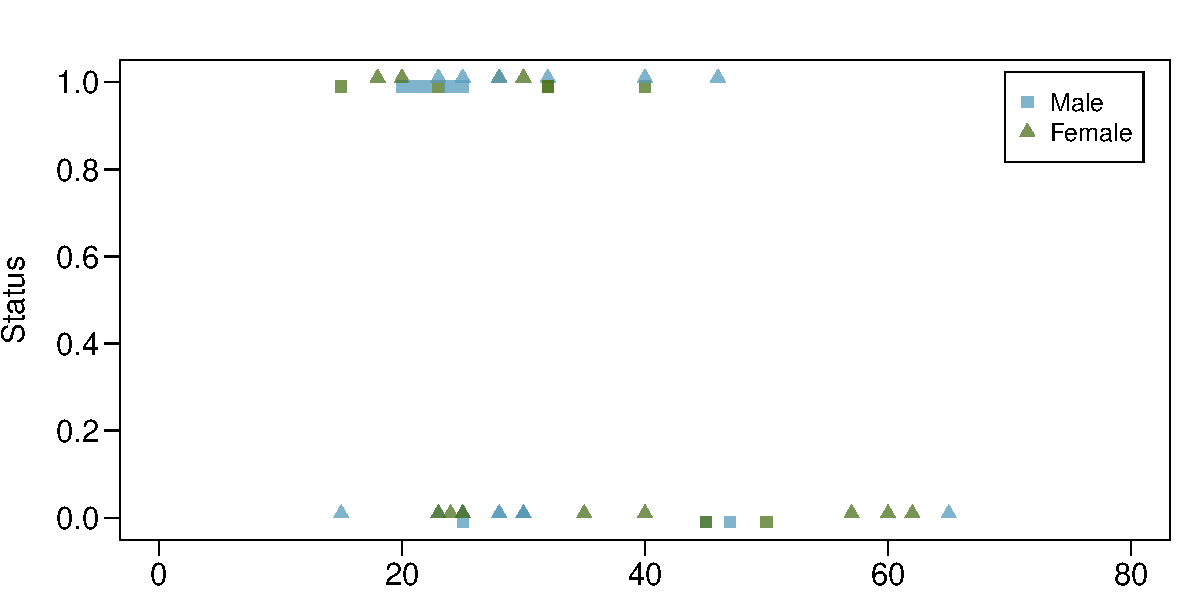
\includegraphics[width=0.8\textwidth]{9-5_logistic_reg/figures/donner/donner_scatter.pdf}}
\only<2>{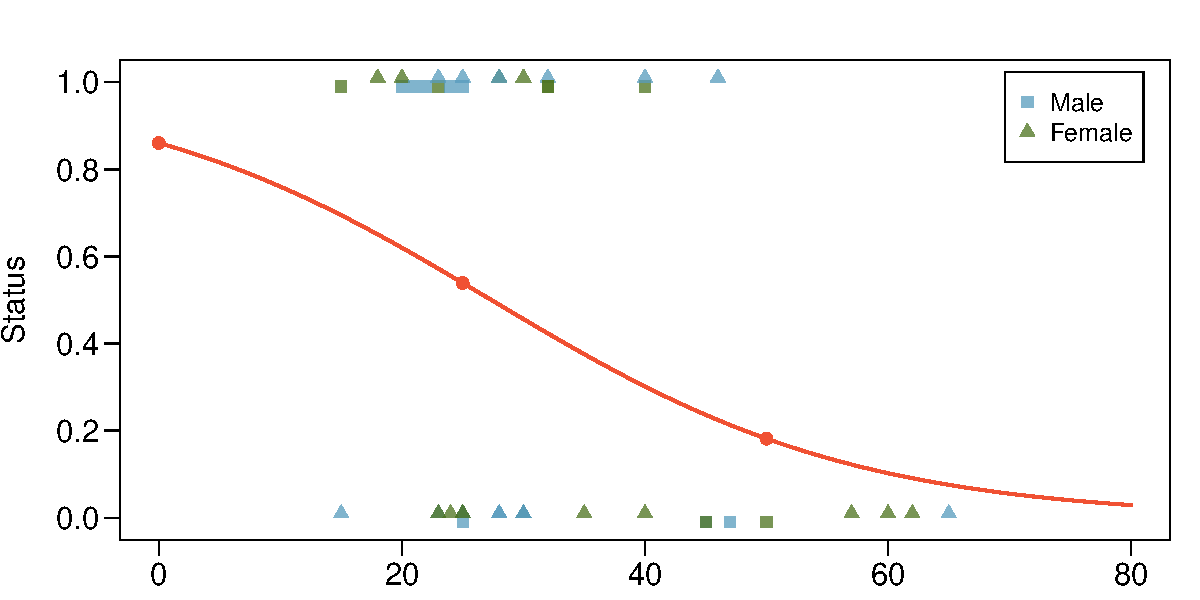
\includegraphics[width=0.8\textwidth]{9-5_logistic_reg/figures/donner/donner_scatter_pred.pdf}}
\end{center}
\end{frame}

%%%%%%%%%%%%%%%%%%%%%%%%%%%%%%%%%%%

\begin{frame}
\frametitle{Example - Donner Party - Interpretation}

{\scriptsize
\begin{center}
\begin{tabular}{rrrrr}
  \hline
 & Estimate & Std. Error & z value & Pr($>$$|$z$|$) \\ 
  \hline
(Intercept) & 1.8185 & 0.9994 & 1.82 & 0.0688 \\ 
  Age & -0.0665 & 0.0322 & -2.06 & 0.0391 \\ 
   \hline
\end{tabular}
\end{center}
}

Simple interpretation is only possible in terms of log odds and log odds ratios for intercept and slope terms.\\

~\\

\hl{Intercept}: The log odds of survival for a party member with an age of 0. From this we can calculate the odds or probability, but additional calculations are necessary.\\

~\\

\hl{Slope}: For a unit increase in age (being 1 year older) how much will the log odds ratio change, not particularly intuitive. More often then not we  care only about sign and relative magnitude. 

\end{frame}

%%%%%%%%%%%%%%%%%%%%%%%%%%%%%%%%%%%

\begin{frame}[fragile]
\frametitle{Example - Donner Party - Interpretation - Slope}

{\scriptsize
\begin{align*}
\log\left(\frac{p_1}{1-p_1}\right) &= 1.8185-0.0665 (x+1) \\
                                   &= 1.8185-0.0665 x-0.0665 \\
\log\left(\frac{p_2}{1-p_2}\right) &= 1.8185-0.0665 x \\
\\
\log\left(\frac{p_1}{1-p_1}\right) - \log\left(\frac{p_2}{1-p_2}\right) &= -0.0665 \\
\log\left(\left. \frac{p_1}{1-p_1} \right/ \frac{p_2}{1-p_2} \right) &= -0.0665 \\
\left. \frac{p_1}{1-p_1} \right/ \frac{p_2}{1-p_2} &= \exp(-0.0665) = 0.94
\end{align*}
}

\end{frame}

%%%%%%%%%%%%%%%%%%%%%%%%%%%%%%%%%%%

\begin{frame}[fragile]
\frametitle{Example - Donner Party - Age and Gender}
\vspace{-3mm}
{\scriptsize
\begin{verbatim}
summary(glm(Status ~ Age + Sex, data=donner, family=binomial))

## Call:
## glm(formula = Status ~ Age + Sex, family = binomial, data = donner)
## 
## Coefficients:
##             Estimate Std. Error z value Pr(>|z|)  
## (Intercept)  1.63312    1.11018   1.471   0.1413  
## Age         -0.07820    0.03728  -2.097   0.0359 *
## SexFemale    1.59729    0.75547   2.114   0.0345 *
## ---
## 
## (Dispersion parameter for binomial family taken to be 1)
## 
##     Null deviance: 61.827  on 44  degrees of freedom
## Residual deviance: 51.256  on 42  degrees of freedom
## AIC: 57.256
## 
## Number of Fisher Scoring iterations: 4
\end{verbatim}
}

\hl{Gender slope}: When the other predictors are held constant this is the log odds ratio between the given level (Female) and the reference level (Male).

\end{frame}

%%%%%%%%%%%%%%%%%%%%%%%%%%%%%%%%%%%

\begin{frame}
\frametitle{Example - Donner Party - Gender Models}

Just like MLR we can plug in gender to arrive at two status vs age models for men and women respectively.\\
~\\

General model:
{\scriptsize
\[\log\left(\frac{p_1}{1-p_1}\right) = 1.63312 + -0.07820\times\text{Age} + 1.59729\times\text{Sex}\]
}

Male model:
{\scriptsize
\begin{align*}
\log\left(\frac{p_1}{1-p_1}\right) &= 1.63312 + -0.07820\times\text{Age} + 1.59729\times\orange{0}\\
                                   &= 1.63312 + -0.07820\times\text{Age}
\end{align*}
}

Female model:
{\scriptsize
\begin{align*}
\log\left(\frac{p_1}{1-p_1}\right) &= 1.63312 + -0.07820\times\text{Age} + 1.59729\times\orange{1}\\
                                   &= 3.23041 + -0.07820\times\text{Age}
\end{align*}
}

\end{frame}

%%%%%%%%%%%%%%%%%%%%%%%%%%%%%%%%%%%

\begin{frame}
\frametitle{Example - Donner Party - Gender Models (cont.)}

\begin{center}
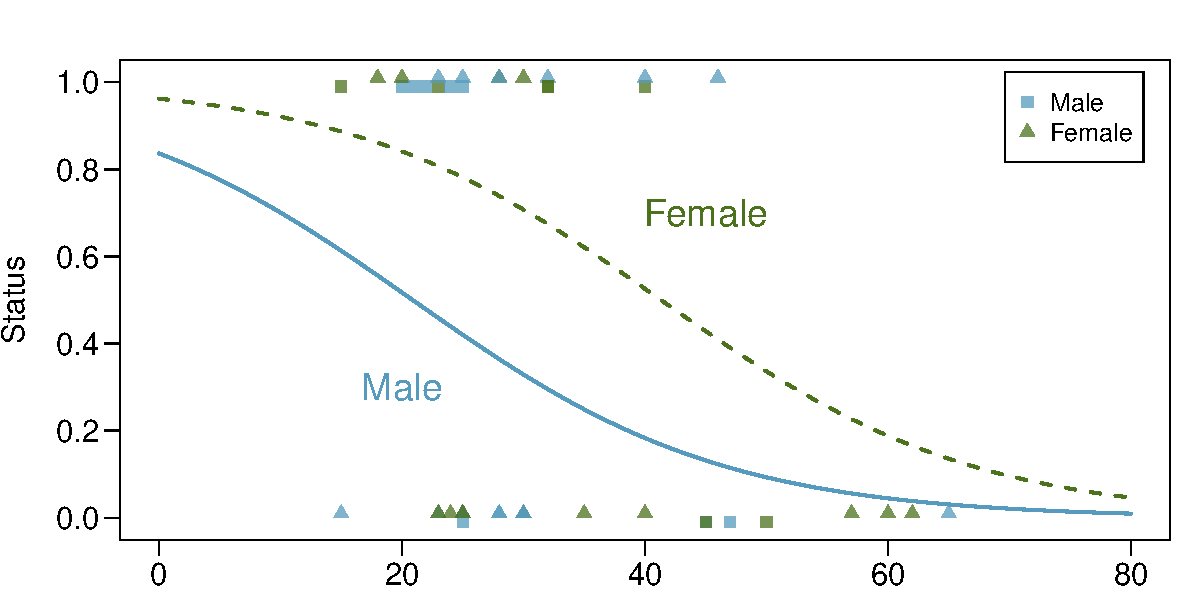
\includegraphics[width=\textwidth]{9-5_logistic_reg/figures/donner/donner_scatter_both.pdf}
\end{center}

\end{frame}

%%%%%%%%%%%%%%%%%%%%%%%%%%%%%%%%%%%

%%%%%%%%%%%%%%%%%%%%%%%%%%%%%%%%%%%

\begin{frame}[fragile,shrink]
\frametitle{Hypothesis test for the whole model}
\vspace{-3mm}
{\scriptsize
\begin{verbatim}
summary(glm(Status ~ Age + Sex, data=donner, family=binomial))

## Call:
## glm(formula = Status ~ Age + Sex, family = binomial, data = donner)
## 
## Coefficients:
##             Estimate Std. Error z value Pr(>|z|)  
## (Intercept)  1.63312    1.11018   1.471   0.1413  
## Age         -0.07820    0.03728  -2.097   0.0359 *
## SexFemale    1.59729    0.75547   2.114   0.0345 *
## ---
## 
## (Dispersion parameter for binomial family taken to be 1)
## 
##     Null deviance: 61.827  on 44  degrees of freedom
## Residual deviance: 51.256  on 42  degrees of freedom
## AIC: 57.256
## 
## Number of Fisher Scoring iterations: 4
\end{verbatim}
}

\pause

\Note{The model output does not include any F-statistic, as a general rule there are not single model hypothesis tests for GLM models.}

\end{frame}

%%%%%%%%%%%%%%%%%%%%%%%%%%%%%%%%%%%

\begin{frame}
\frametitle{Hypothesis tests for a coefficient}

\begin{center}
\begin{tabular}{rrrrr}
  \hline
 & Estimate & Std. Error & z value & Pr($>$$|$z$|$) \\ 
  \hline
(Intercept) & 1.6331 & 1.1102 & 1.47 & 0.1413 \\ 
  Age & -0.0782 & 0.0373 & -2.10 & 0.0359 \\ 
  SexFemale & 1.5973 & 0.7555 & 2.11 & 0.0345 \\ 
   \hline
\end{tabular}
\end{center}

We are however still able to perform inference on individual coefficients, the basic setup is exactly the same as what we've seen before except we use a Z test.\\

~\\

\Note{The only tricky bit, which is way beyond the scope of this course, is how the standard error is calculated.}

\end{frame}

%%%%%%%%%%%%%%%%%%%%%%%%%%%%%%%%%%%

\begin{frame}
\frametitle{Testing for the slope of Age}

{\small
\begin{center}
\begin{tabular}{rrrrr}
  \hline
            & Estimate & Std. Error & z value & Pr($>$$|$z$|$) \\ 
  \hline
(Intercept) & 1.6331  & 1.1102 & 1.47 & 0.1413 \\ 
        Age & \orange{-0.0782} & \green{0.0373} & \orange{-2.10} & \textcolor{blue}{0.0359} \\ 
  SexFemale & 1.5973  & 0.7555 & 2.11 & 0.0345 \\ 
   \hline
\end{tabular}
\end{center}
}

\pause

\begin{align*}
H_0:~& \beta_{age} = 0 \\
H_A:~& \beta_{age} \ne 0
\end{align*}

\pause

\begin{align*}
Z &= \frac{\hat{\beta_{age}} - \beta_{age}}{SE_{age}} 
   = \frac{\orange{-0.0782} - 0}{\green{0.0373}} = \orange{-2.10} \\
\\
\text{p-value} &= P(|Z| > \orange{2.10}) = P(Z>\orange{2.10})+P(Z<\orange{-2.10})\\
               &= 2\times 0.0178 = \textcolor{blue}{0.0359}
\end{align*}

\end{frame}

%%%%%%%%%%%%%%%%%%%%%%%%%%%%%%%%%%%

%%%%%%%%%%%%%%%%%%%%%%%%%%%%%%%%%%%

\begin{frame}
\frametitle{Confidence interval for age slope coefficient}

\begin{center}
\begin{tabular}{rrrrr}
  \hline
 & Estimate & Std. Error & z value & Pr($>$$|$z$|$) \\ 
  \hline
(Intercept) & 1.6331 & 1.1102 & 1.47 & 0.1413 \\ 
  Age & -0.0782 & 0.0373 & -2.10 & 0.0359 \\ 
  SexFemale & 1.5973 & 0.7555 & 2.11 & 0.0345 \\ 
   \hline
\end{tabular}
\end{center}

Remember, the interpretation for a slope is the change in log odds ratio per unit change in the predictor.\\
~\\

\pause

Log odds ratio:
\[ CI = PE \pm CV \times SE = -0.0782 \pm 1.96 \times 0.0373 = (-0.1513,  -0.0051) \]

\pause

Odds ratio:
\[ \exp(CI) = (\exp{-0.1513}, \exp{-0.0051}) = (0.8596 0.9949) \]


\end{frame}


%%%%%%%%%%%%%%%%%%%%%%%%%%%%%%%%%%%

\subsection{Additional Example}

%%%%%%%%%%%%%%%%%%%%%%%%%%%%%%%%%%%


\begin{frame}
\frametitle{Example - Birdkeeping and Lung Cancer}

A 1972 - 1981 health survey in The Hague, Netherlands, discovered an association between keeping pet birds and increased risk of lung cancer. To investigate birdkeeping as a risk factor, researchers conducted a case-control study of patients in 1985 at four hospitals in The Hague (population 450,000). They identified 49 cases of lung cancer among the patients who were registered with a general practice, who were age 65 or younger and who had resided in the city since 1965. They also selected 98 controls from a population of residents having the same general age structure.


\vfill

{\tiny From \textit{Ramsey, F.L. and Schafer, D.W. (2002). The Statistical Sleuth: A Course in Methods of Data Analysis (2nd ed)}}
\end{frame}

%%%%%%%%%%%%%%%%%%%%%%%%%%%%%%%%%%%

\begin{frame}
\frametitle{Example - Birdkeeping and Lung Cancer - Data}

\begin{tabular}{rllllrrr}
  \hline
    & \var{LC} & \var{FM} & \var{SS} & \var{BK} & \var{AG} & \var{YR} & \var{CD} \\ 
  \hline
  1 & LungCancer & Male & Low & Bird & 37.00 & 19.00 & 12.00 \\ 
  2 & LungCancer & Male & Low & Bird & 41.00 & 22.00 & 15.00 \\ 
  3 & LungCancer & Male & High & NoBird & 43.00 & 19.00 & 15.00 \\ 
\vdots & ~~~~~~\vdots & ~~~\vdots & ~~\vdots & ~~~\vdots & \vdots~~~ & \vdots~~~ & \vdots~~~ \\
147 & NoCancer & Female & Low & NoBird & 65.00 & 7.00 & 2.00 \\ 
   \hline
\end{tabular}

~\\

{\small
\begin{center}
\begin{tabular}{ll}
\var{LC} & Whether subject has lung cancer \\
\var{FM} & Sex of subject \\
\var{SS} & Socioeconomic status \\
\var{BK} & Indicator for birdkeeping \\
\var{AG} & Age of subject (years) \\
\var{YR} & Years of smoking prior to diagnosis or examination \\
\var{CD} & Average rate of smoking (cigarettes per day)
\end{tabular}
\end{center}
}

\Note{NoCancer is the reference response (0 or failure), LungCancer is the non-reference response (1 or success) - this matters for interpretation.}

\end{frame}

%%%%%%%%%%%%%%%%%%%%%%%%%%%%%%%%%%%

\begin{frame}
\frametitle{Example - Birdkeeping and Lung Cancer - EDA}

\begin{center}
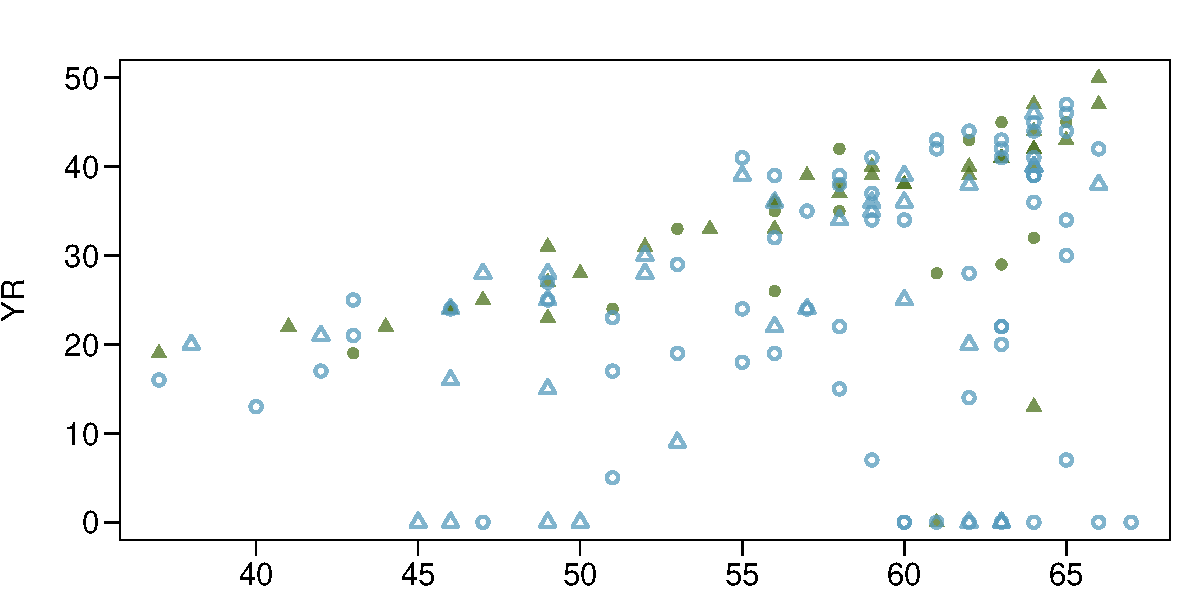
\includegraphics[width=0.8\textwidth]{9-5_logistic_reg/figures/birds/birds.pdf}
\end{center}

{\scriptsize
\begin{center}
\begin{tabular}{r|cc}
               & Bird             & No Bird \\
\hline               
Lung Cancer    & \textcolor{oiG}{$\blacktriangle$} & \textcolor{oiG}{$\bullet$} \\
No Lung Cancer & \textcolor{oiB}{$\triangle$}      & \textcolor{oiB}{$\circ$}
\end{tabular}
\end{center}
}

 
 
\end{frame}

%%%%%%%%%%%%%%%%%%%%%%%%%%%%%%%%%%%

\begin{frame}[fragile]
\frametitle{Example - Birdkeeping and Lung Cancer - Model}

\vspace{-5mm}

{\scriptsize
\begin{verbatim}
summary(glm(LC ~ FM + SS + BK + AG + YR + CD, data=bird, family=binomial))

## Call:
## glm(formula = LC ~ FM + SS + BK + AG + YR + CD, family = binomial, 
##     data = bird)
## 
## Coefficients:
##             Estimate Std. Error z value Pr(>|z|)    
## (Intercept) -1.93736    1.80425  -1.074 0.282924    
## FMFemale     0.56127    0.53116   1.057 0.290653    
## SSHigh       0.10545    0.46885   0.225 0.822050    
## BKBird       1.36259    0.41128   3.313 0.000923 ***
## AG          -0.03976    0.03548  -1.120 0.262503    
## YR           0.07287    0.02649   2.751 0.005940 ** 
## CD           0.02602    0.02552   1.019 0.308055    
## 
## (Dispersion parameter for binomial family taken to be 1)
## 
##     Null deviance: 187.14  on 146  degrees of freedom
## Residual deviance: 154.20  on 140  degrees of freedom
## AIC: 168.2
## 
## Number of Fisher Scoring iterations: 5
\end{verbatim}
}

\end{frame}

%%%%%%%%%%%%%%%%%%%%%%%%%%%%%%%%%%%

\begin{frame}
\frametitle{Example - Birdkeeping and Lung Cancer - Interpretation}

\vspace{-5mm}

{\scriptsize
\begin{center}
\begin{tabular}{rrrrr}
  \hline
 & Estimate & Std. Error & z value & Pr($>$$|$z$|$) \\ 
  \hline
(Intercept) & -1.9374 & 1.8043 & -1.07 & 0.2829 \\ 
  FMFemale  & 0.5613 & 0.5312 & 1.06 & 0.2907 \\ 
  SSHigh    & 0.1054 & 0.4688 & 0.22 & 0.8221 \\
\rowcolor{gray}
  BKBird    & 1.3626 & 0.4113 & 3.31 & 0.0009 \\ 
  AG        & -0.0398 & 0.0355 & -1.12 & 0.2625 \\ 
\rowcolor{gray}
  YR        & 0.0729 & 0.0265 & 2.75 & 0.0059 \\ 
  CD        & 0.0260 & 0.0255 & 1.02 & 0.3081 \\ 
   \hline
\end{tabular}
\end{center}
}

\pause

Keeping all other predictors constant then,
\begin{itemize}
\pause
\item The odds ratio of getting lung cancer for bird keepers vs non-bird keepers is $\exp(1.3626) = 3.91$.
\pause
\item The odds ratio of getting lung cancer for an additional year of smoking is $\exp(0.0729) = 1.08$.
\end{itemize}

\end{frame}

%%%%%%%%%%%%%%%%%%%%%%%%%%%%%%%%%%%

\begin{frame}
\frametitle{What do the numbers not mean ...}

The most common mistake made when interpreting logistic regression is to treat an odds ratio as a ratio of probabilities.\\

~\\ \pause

Bird keepers are \emph{not} 4x more likely to develop lung cancer than non-bird keepers.

~\\ \pause

This is the difference between relative risk and an odds ratio.


\[RR = \frac{P(\text{disease} | \text{exposed})}{P(\text{disease} | \text{unexposed})} \]

\[OR = \frac{P(\text{disease} | \text{exposed}) / [1-P(\text{disease} | \text{exposed})]}{P(\text{disease} | \text{unexposed})/[1-P(\text{disease} | \text{unexposed})]} \]


\end{frame}

%%%%%%%%%%%%%%%%%%%%%%%%%%%%%%%%%%%

\begin{frame}
\frametitle{Back to the birds}

What is probability of lung cancer in a bird keeper if we knew that $P(\text{lung cancer}|\text{no birds}) = 0.05$?

\begin{align*}
OR &= \frac{P(\text{lung cancer} | \text{birds}) / [1-P(\text{lung cancer} | \text{birds})]}{P(\text{lung cancer} | \text{no birds})/[1-P(\text{lung cancer} | \text{no birds})]} \\
\\
   &= \frac{P(\text{lung cancer} | \text{birds}) / [1-P(\text{lung cancer} | \text{birds})]}{0.05/[1-0.05]} = 3.91
\end{align*}

\pause

\[ P(\text{lung cancer} | \text{birds}) =  \frac{3.91 \times \frac{0.05}{0.95}}{1+3.91 \times \frac{0.05}{0.95}} = 0.171\]

\pause

\[ RR = P(\text{lung cancer} | \text{birds}) / P(\text{lung cancer} | \text{no birds}) = 0.171 / 0.05 = 3.41\]

\end{frame}

%%%%%%%%%%%%%%%%%%%%%%%%%%%%%%%%%%

\begin{frame}
\frametitle{Bird OR Curve}

\vspace{-8mm}

\begin{center}
\only<1|handout:0>{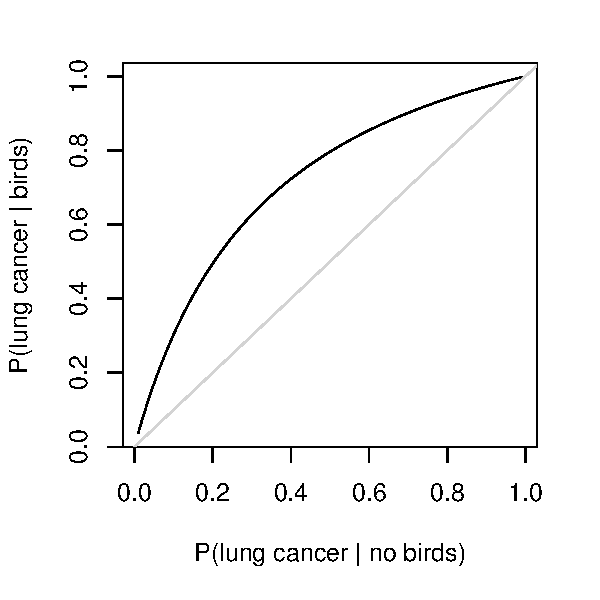
\includegraphics[width=0.7\textwidth]{9-5_logistic_reg/figures/birds/OR1.pdf}}
\only<2|handout:0>{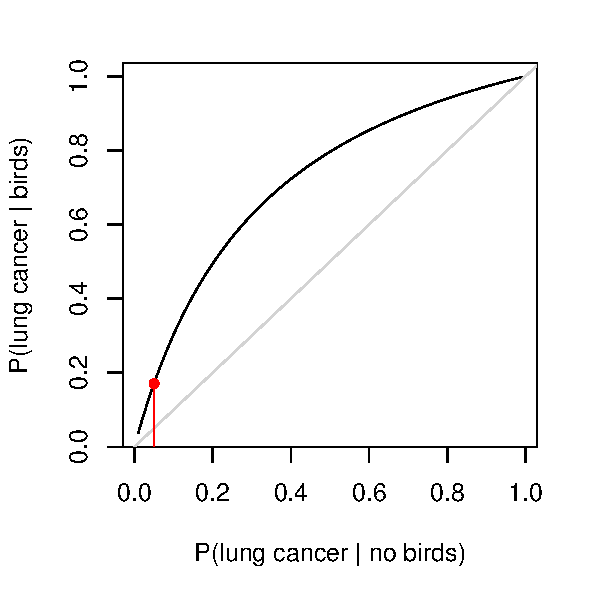
\includegraphics[width=0.7\textwidth]{9-5_logistic_reg/figures/birds/OR2.pdf}}
\only<3|handout:1>{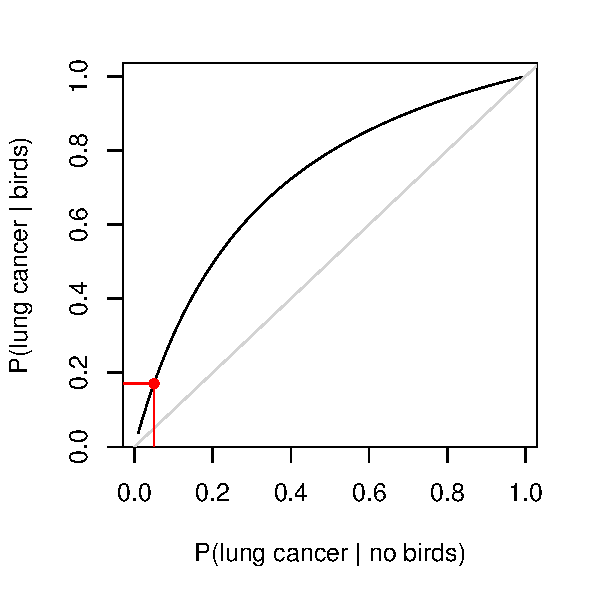
\includegraphics[width=0.7\textwidth]{9-5_logistic_reg/figures/birds/OR3.pdf}}
\end{center}

\end{frame}

%%%%%%%%%%%%%%%%%%%%%%%%%%%%%%%%%%

\begin{frame}
\frametitle{OR Curves}

\vspace{-5mm}

\begin{center}
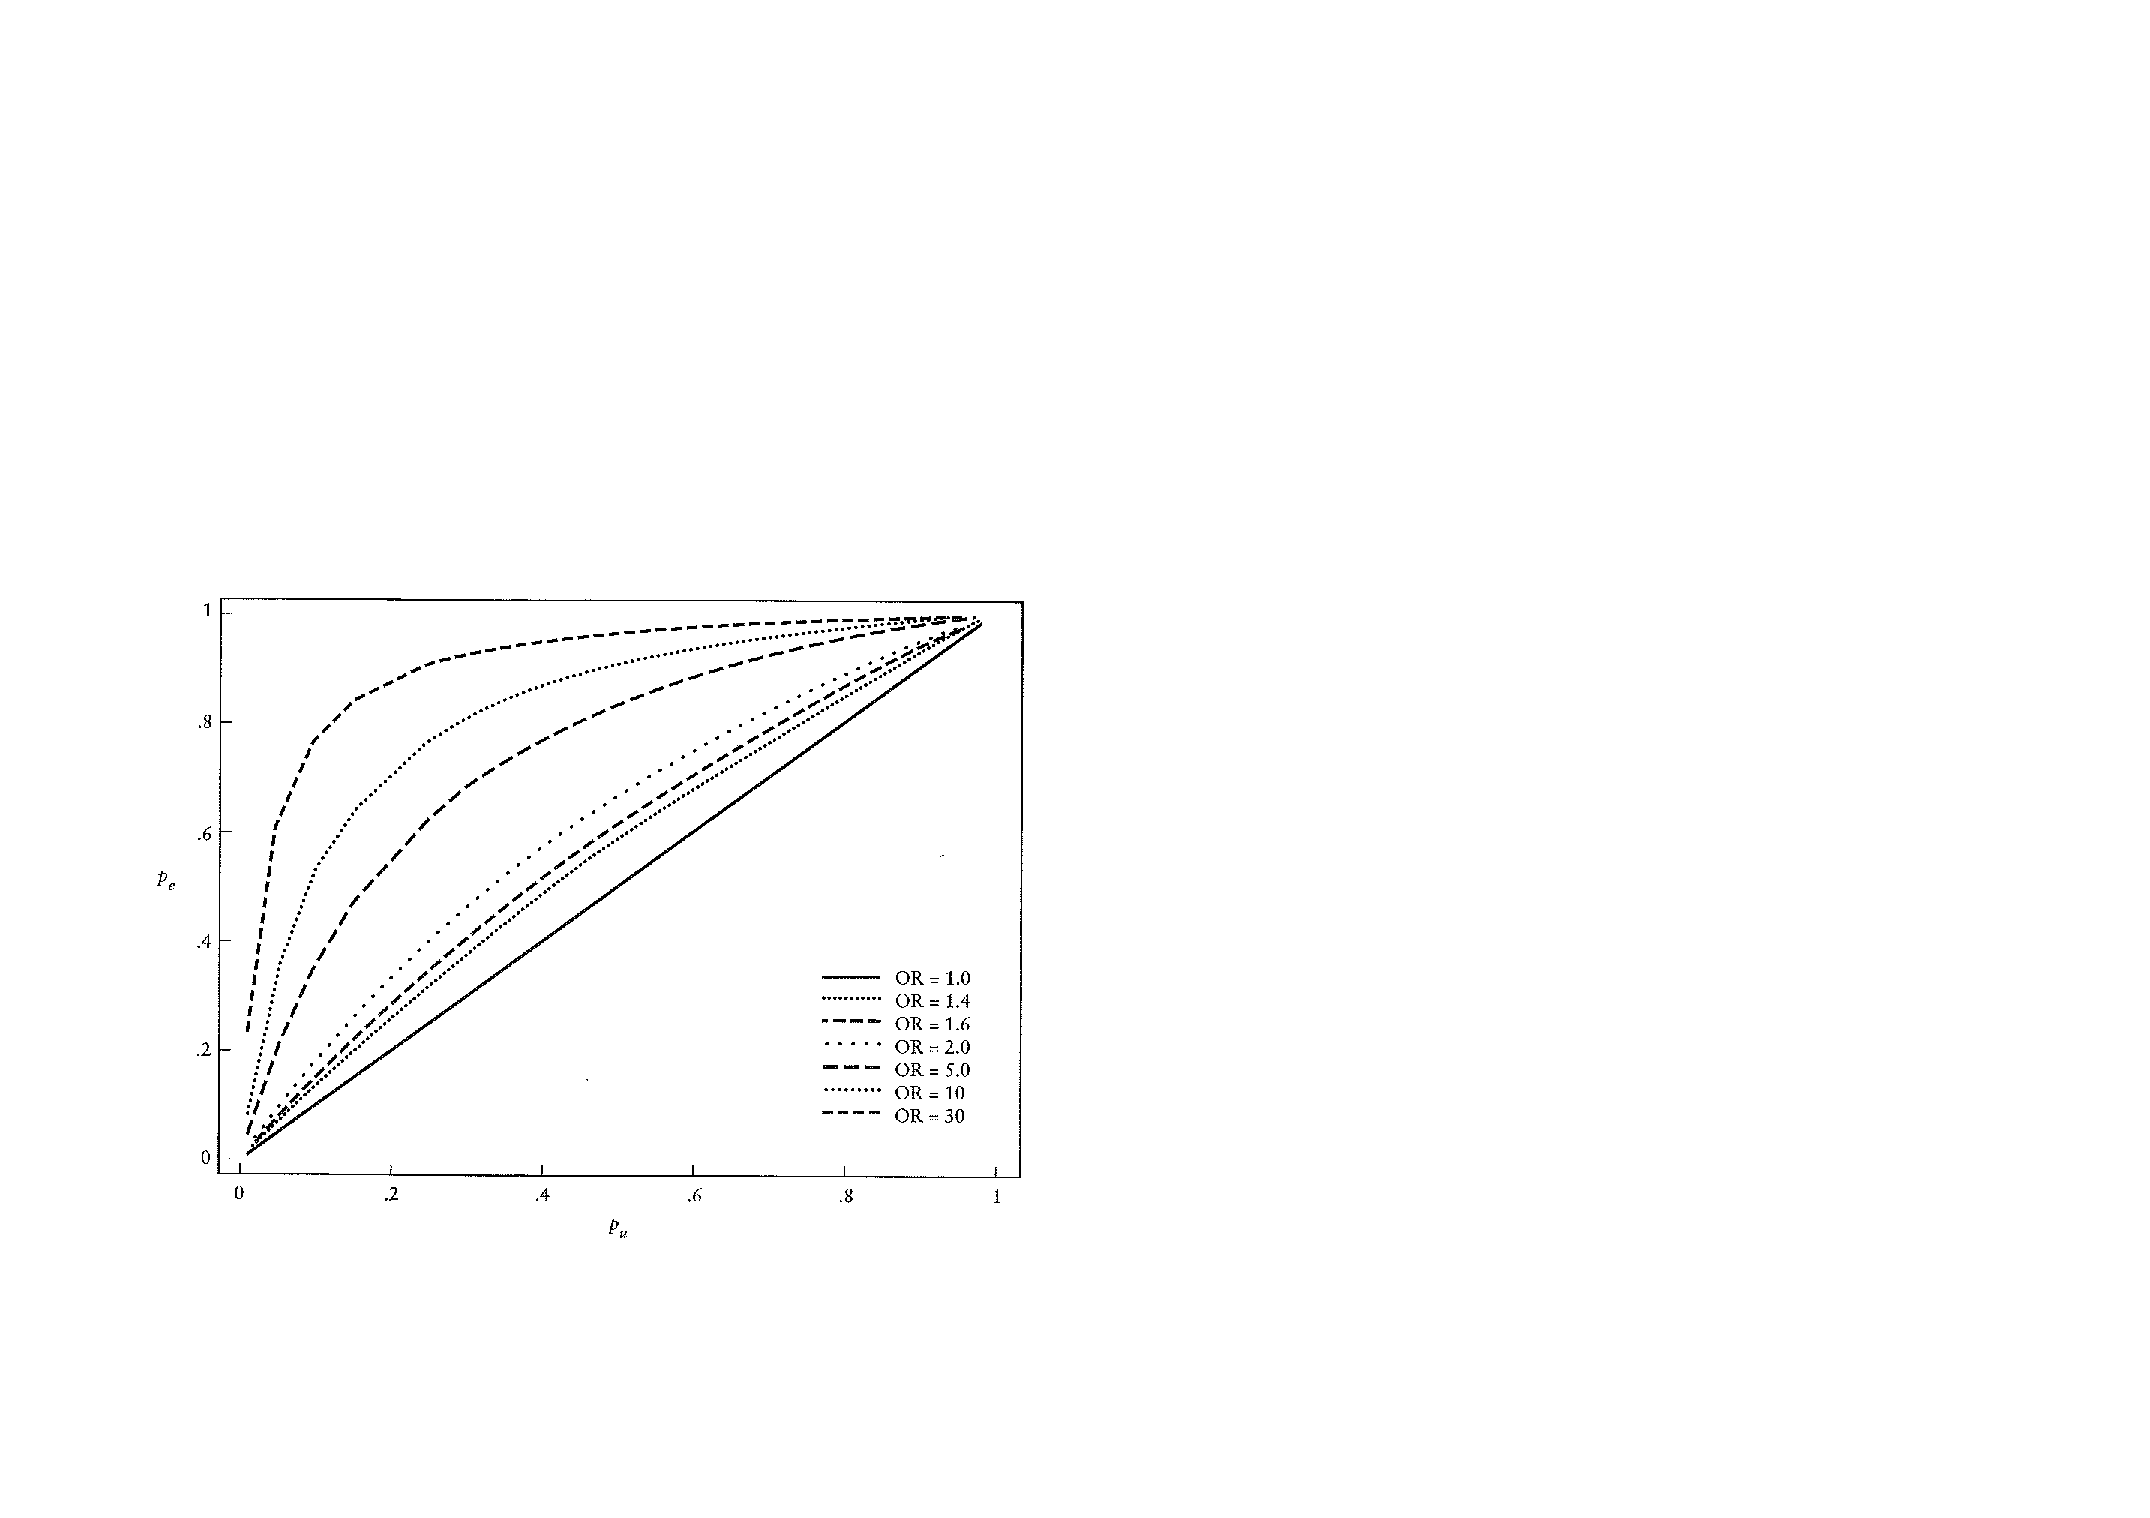
\includegraphics[width=0.85\textwidth]{9-5_logistic_reg/figures/all_OR.pdf}
\end{center}

\end{frame}

%%%%%%%%%%%%%%%%%%%%%%%%%%%%%%%%%%

\subsection{Sensitivity and Specificity}

%%%%%%%%%%%%%%%%%%%%%%%%%%%%%%%%%%%

\begin{frame}
\frametitle{(An old) Example - \emph{House}}

If you've ever watched the TV show \emph{House} on Fox, you know that Dr. House regularly states, ``It's never lupus." \\
\vspace{3mm}
Lupus is a medical phenomenon where antibodies that are supposed to attack foreign cells to prevent infections instead see plasma proteins as foreign bodies, leading to a high risk of blood clotting. It is believed that 2\% of the population suffer from this disease. \\
\vspace{3mm}
The test for lupus is very accurate if the person actually has lupus, however is very inaccurate if the person does not. More specifically, the test is 98\% accurate if a person actually has the disease. The test is 74\% accurate if a person does not have the disease. \\
\vspace{3mm}
Is Dr. House correct even if someone tests positive for Lupus? 

\end{frame}

%%%%%%%%%%%%%%%%%%%%%%%%%%%%%%%%%%

\begin{frame}
\frametitle{(An old) Example - \emph{House}}

\begin{center}
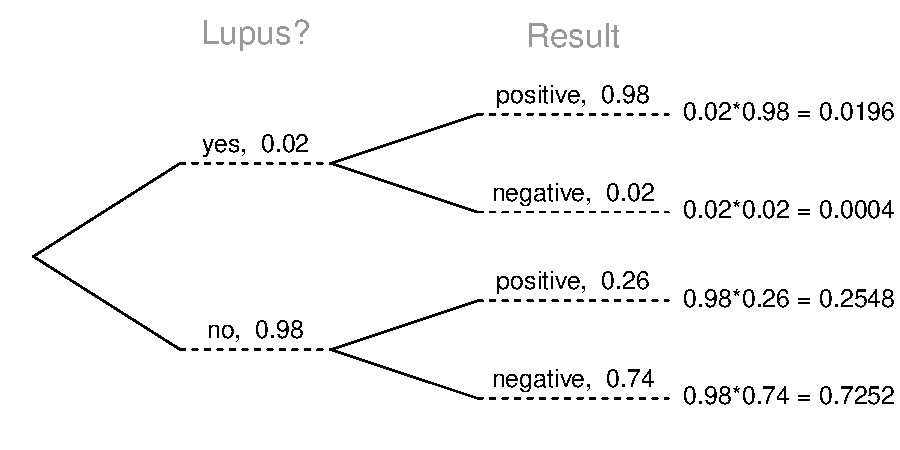
\includegraphics[width=0.8\textwidth]{9-5_logistic_reg/figures/tree_lupus.pdf}
\end{center}

{\footnotesize
\begin{align*}
P(\text{Lupus} | +)  &= \frac{P(+,\text{Lupus})}{P(+,\text{Lupus})+P(+,\text{No Lupus})} \\
                     &= \frac{0.0196}{0.0196+0.2548} = 0.0714
\end{align*}
}
\end{frame}

%%%%%%%%%%%%%%%%%%%%%%%%%%%%%%%%%%

\begin{frame}
\frametitle{Testing for lupus}
It turns out that testing for Lupus is actually quite complicated, a diagnosis usually relies on the outcome of multiple tests, often including: a complete blood count, an erythrocyte sedimentation rate, a kidney and liver assessment, a urinalysis, and or an antinuclear antibody (ANA) test.\\
~\\
It is important to think about what is involved in each of these tests (e.g. deciding if complete blood count is high or low) and how each of the individual tests and related decisions plays a role in the overall decision of diagnosing a patient with lupus.\\

\end{frame}

%%%%%%%%%%%%%%%%%%%%%%%%%%%%%%%%%%

\begin{frame}
\frametitle{Testing for lupus}

At some level we can view a diagnosis as a binary decision (lupus or no lupus) that involves the complex integration of various explanatory variables.\\
~\\
The example does not give us any information about how a diagnosis is made, but what it does give us is just as important - the sensitivity and the specificity of the test. These values are critical for our understanding of what a positive or negative test result actually means.

\end{frame}

%%%%%%%%%%%%%%%%%%%%%%%%%%%%%%%%%%

\begin{frame}
\frametitle{Sensitivity and Specificity}

\hl{Sensitivity} - measures a tests ability to identify positive results.
\[P(\text{Test }+~|~\text{Conditon }+) = P(+ | \text{lupus}) = 0.98\]

\hl{Specificity} - measures a tests ability to identify negative results.

\[P(\text{Test }-~|~\text{Condition }-) = P(- | \text{no lupus}) = 0.74\]

\pause
\vspace{1cm}

It is illustrative to think about the extreme cases - what is the sensitivity and specificity of a test that always returns a positive result? What about a test that always returns a negative result?

\end{frame}

%%%%%%%%%%%%%%%%%%%%%%%%%%%%%%%%%%

\begin{frame}
\frametitle{Sensitivity and Specificity (cont.)}

\vspace{-5mm}

\begin{center}
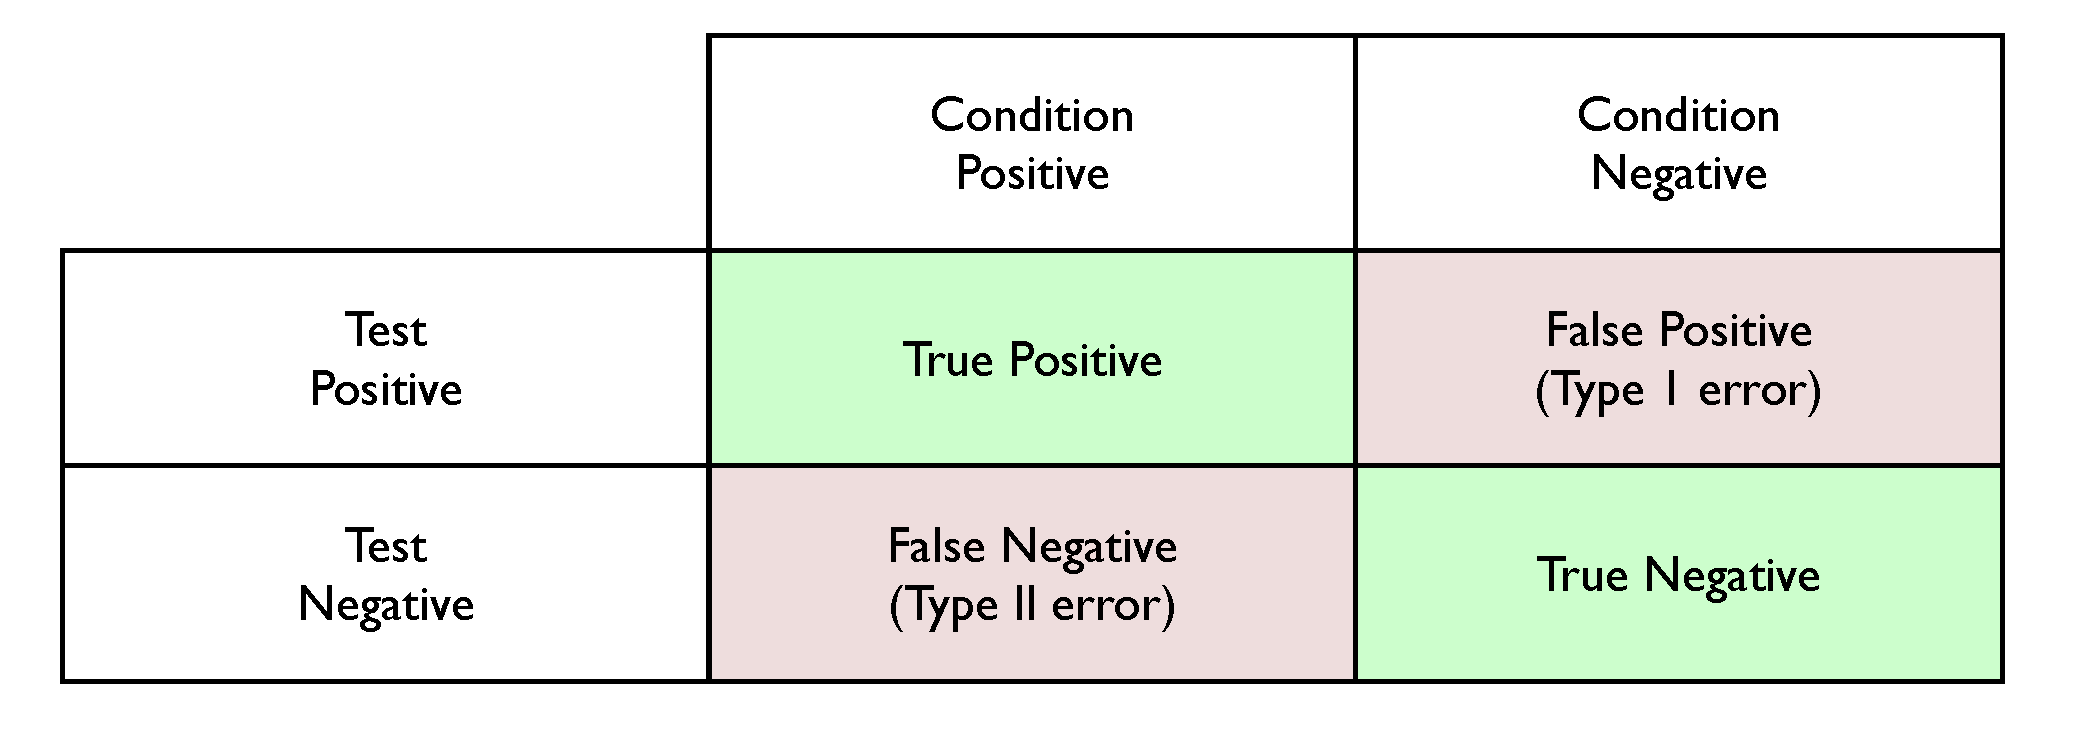
\includegraphics[width=\textwidth]{9-5_logistic_reg/figures/SenSpec.pdf}
\end{center}

\vspace{-9mm}

{\small
\begin{align*}
\only<2->{\text{\hl{Sensitivity}} &= P(\text{Test }+~|~\text{Condition }+)} \only<3->{ = TP / (TP + FN)} \\
\only<4->{\text{\hl{Specificity}} &= P(\text{Test }-~|~\text{Condition }-)} \only<5->{ = TN / (FP + TN)}\\
\only<6->{\text{\hl{False negative rate} (\hl{$\beta$})}  &= P(\text{Test }-~|~\text{Condition }+)} \only<7->{= FN / (TP + FN)} \\
\only<8->{\text{\hl{False positive rate} (\hl{$\alpha$})} &= P(\text{Test }+~|~\text{Condition }-)} \only<9->{= FP / (FP + TN)}
\end{align*}

\vspace{-2mm}

\begin{align*}
\only<10->{
\text{\hl{Sensitivity}} &= 1 - \text{\hl{False negative rate}} = \text{Power}\\
\text{\hl{Specificity}} &= 1 - \text{\hl{False positive rate}}
}
\end{align*}
}

\end{frame}

%%%%%%%%%%%%%%%%%%%%%%%%%%%%%%%%%%

\begin{frame}
\frametitle{So what?}

Clearly it is important to know the Sensitivity and Specificity of test (and or the false positive and false negative rates). Along with the incidence of the disease (e.g. $P(\text{lupus})$) these values are necessary to calculate important quantities like $P(\text{lupus} | + )$. \\
~\\
Additionally, our brief foray into power analysis before the first midterm should also give you an idea about the trade offs that are inherent in minimizing false positive and false negative rates (increasing power required either increasing $\alpha$ or $n$).\\
~\\
How should we use this information when we are trying to come up with a decision?
\end{frame}

%%%%%%%%%%%%%%%%%%%%%%%%%%%%%%%%%%%

\subsection{ROC curves}

%%%%%%%%%%%%%%%%%%%%%%%%%%%%%%%%%%%

\begin{frame}
\frametitle{Back to Spam}

In lab this week, we examined a data set of emails where we were interesting in identifying the spam messages. We examined different logistic regression models to evaluate how different predictors influenced the probability of a message being spam.\\

~\\

These models can also be used to assign probabilities to incoming messages (this is equivalent to prediction in the case of SLR / MLR). However, if we were designing a spam filter this would only be half of the battle, we would also need to use these probabilities to make a decision about which emails get flagged as spam.\\

~\\ \pause

While not the only possible solution, we will consider a simple approach where we choose a threshold probability and any email that exceeds that probability is flagged as spam.

\end{frame}


%%%%%%%%%%%%%%%%%%%%%%%%%%%%%%%%%%

\begin{frame}
\frametitle{Picking a threshold}

\vspace{-5mm}

\begin{center}
\only<1-2|handout:0>{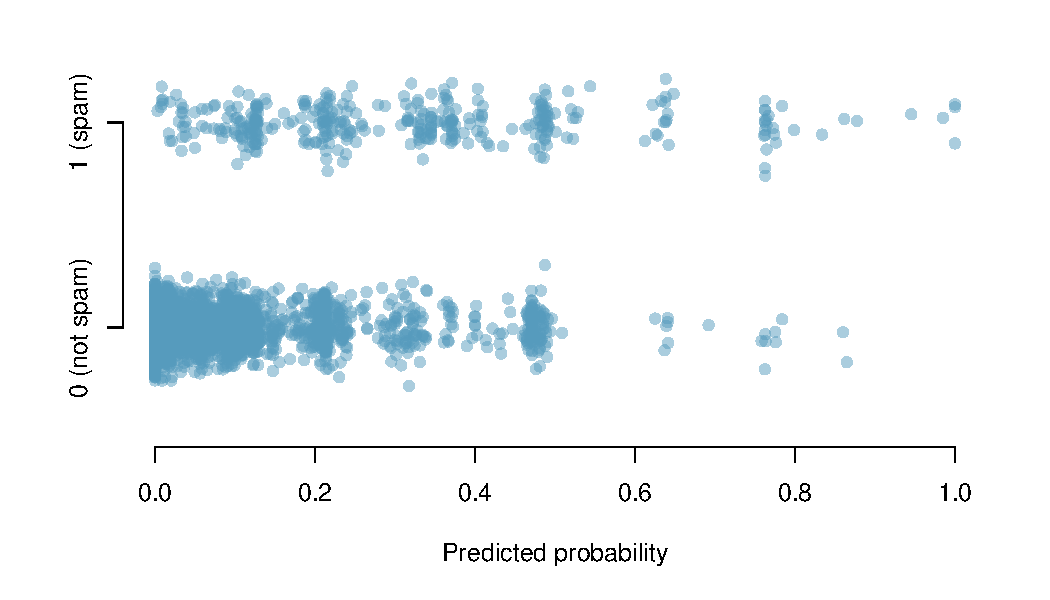
\includegraphics[width=\textwidth]{9-5_logistic_reg/figures/spam/spam1.pdf}}
\only<3|handout:0>{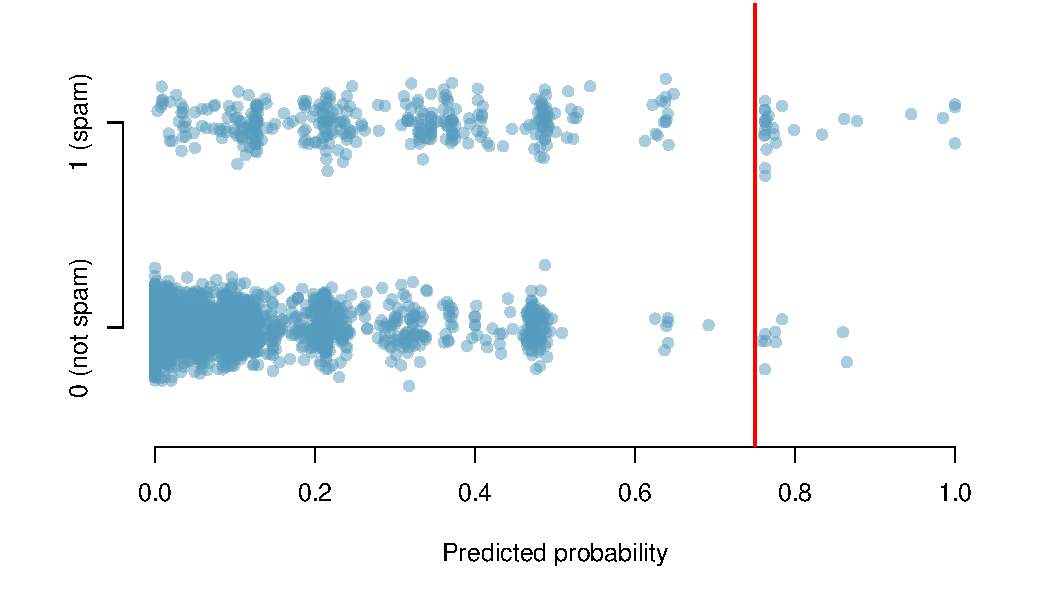
\includegraphics[width=\textwidth]{9-5_logistic_reg/figures/spam/spam2.pdf}}
\only<4|handout:0>{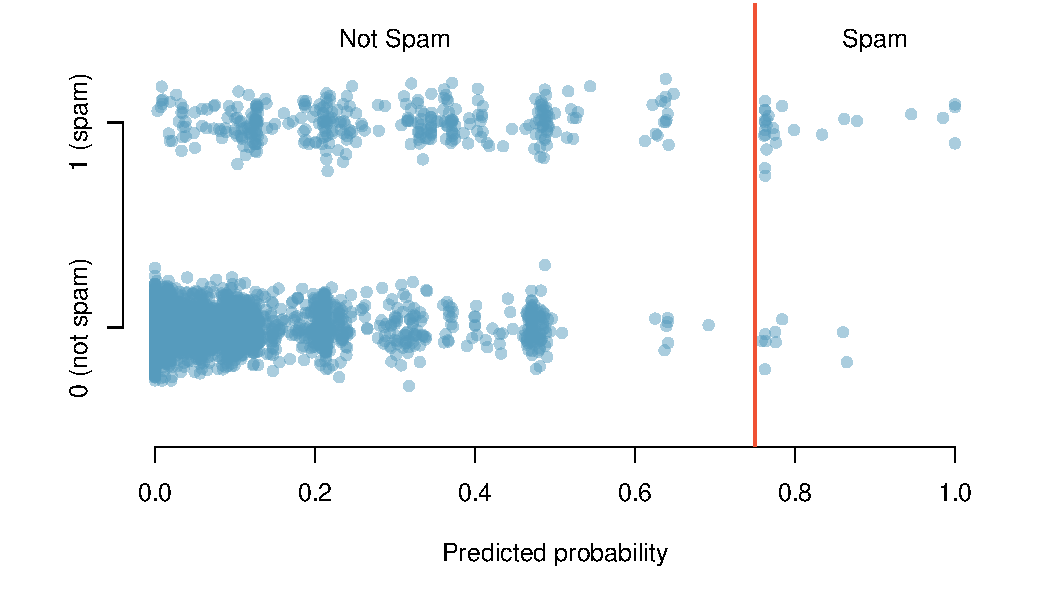
\includegraphics[width=\textwidth]{9-5_logistic_reg/figures/spam/spam3.pdf}}
\only<5|handout:0>{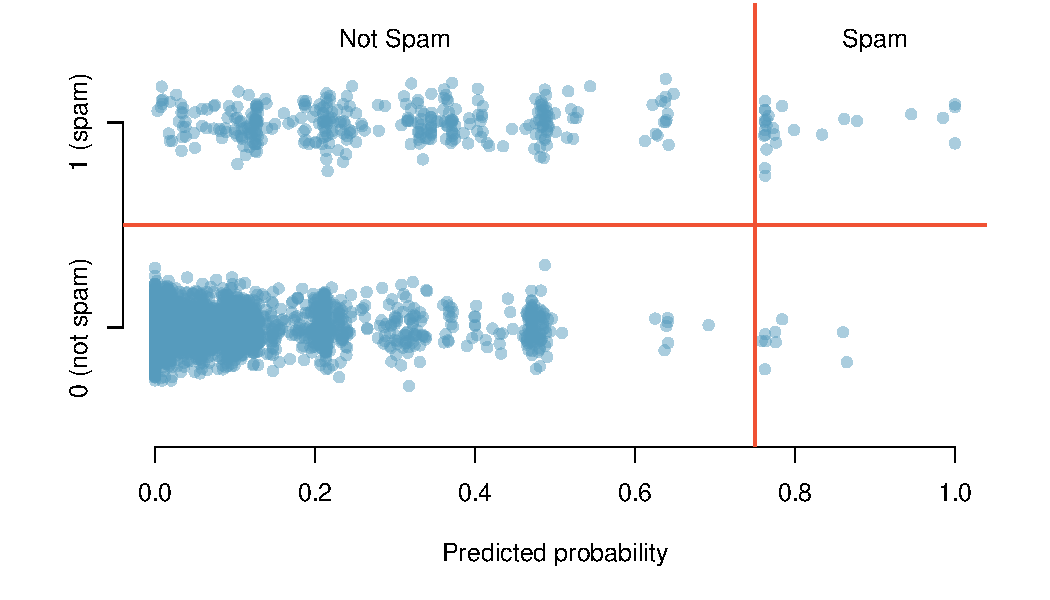
\includegraphics[width=\textwidth]{9-5_logistic_reg/figures/spam/spam4.pdf}}
\only<6|handout:1>{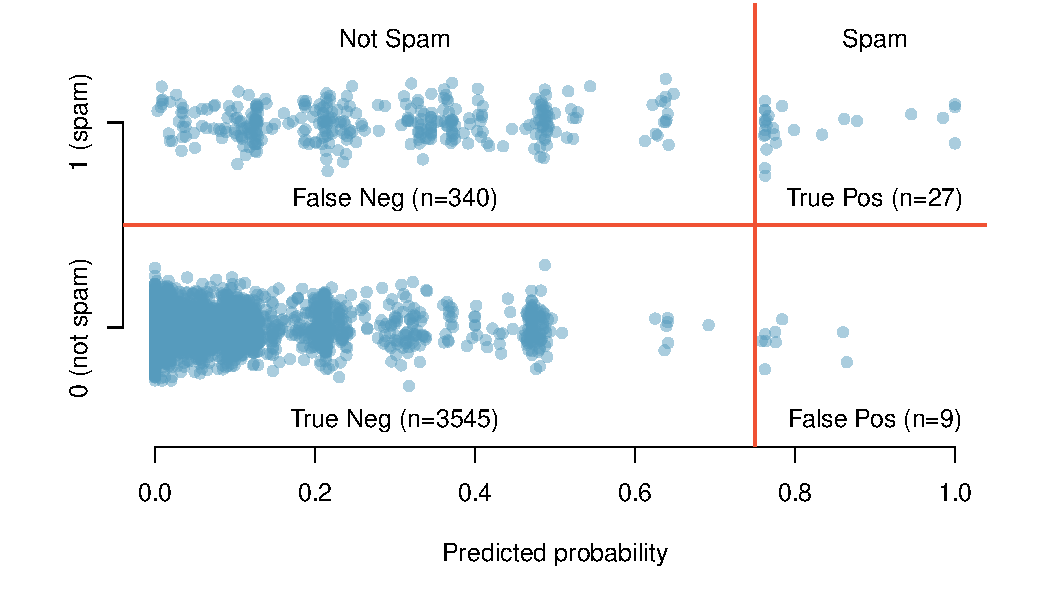
\includegraphics[width=\textwidth]{9-5_logistic_reg/figures/spam/spam5.pdf}}
\end{center}

\vspace{-7mm}

\begin{center}
\only<2->{Lets see what happens if we pick our threshold to be \orange{0.75}.}
\end{center}

\end{frame}

%%%%%%%%%%%%%%%%%%%%%%%%%%%%%%%%%%

\begin{frame}
\frametitle{Consequences of picking a threshold}

For our data set picking a threshold of 0.75 gives us the following results:
\vspace{-1.5mm}
\begin{align*}
FN = 340 &\qquad TP = 27 \\
TN = 3545 &\qquad FP = 9
\end{align*}

\pause
What are the sensitivity and specificity for this particular decision rule?
\pause

\soln{
\begin{align*}
\text{Sensitivity} & = TP / (TP + FN) = 27 / (27+340) = 0.073 \\
\text{Specificity} & = TN / (FP + TN) = 3545 / (9+3545) = 0.997 \\
\end{align*}
}

\end{frame}

%%%%%%%%%%%%%%%%%%%%%%%%%%%%%%%%%%

\begin{frame}
\frametitle{Trying other thresholds}

\vspace{-5mm}

\begin{center}
\only<1|handout:1>{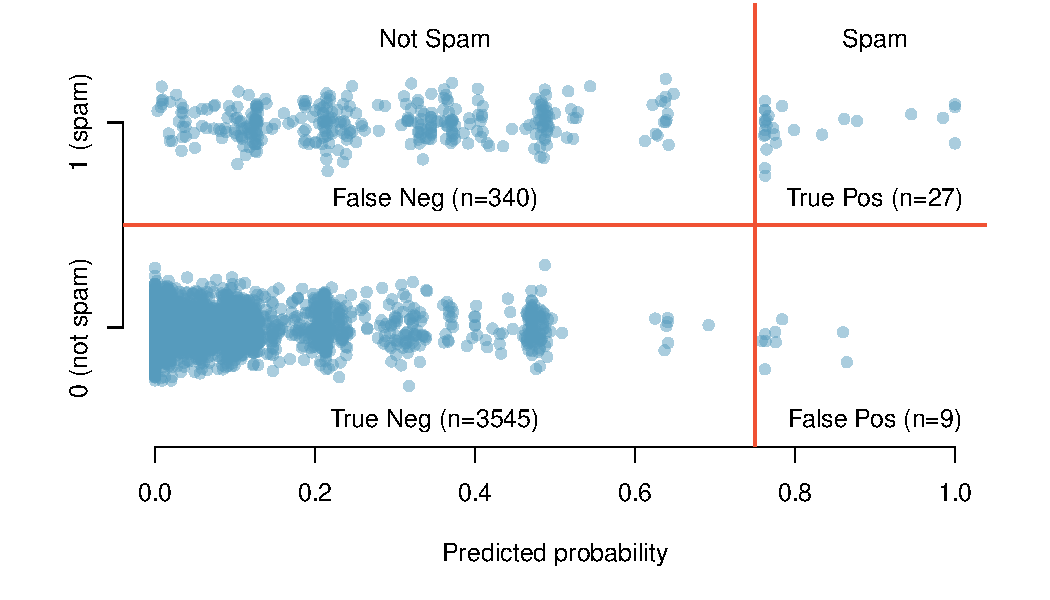
\includegraphics[width=0.9\textwidth]{9-5_logistic_reg/figures/spam/spam5-1.pdf}}
\only<2|handout:0>{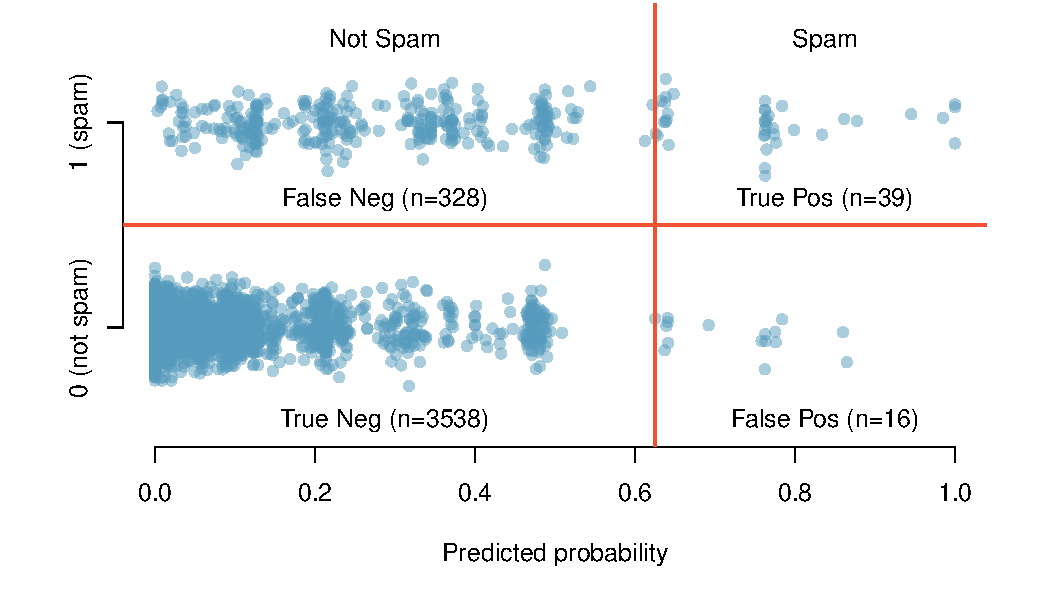
\includegraphics[width=0.9\textwidth]{9-5_logistic_reg/figures/spam/spam5-2.pdf}}
\only<3|handout:0>{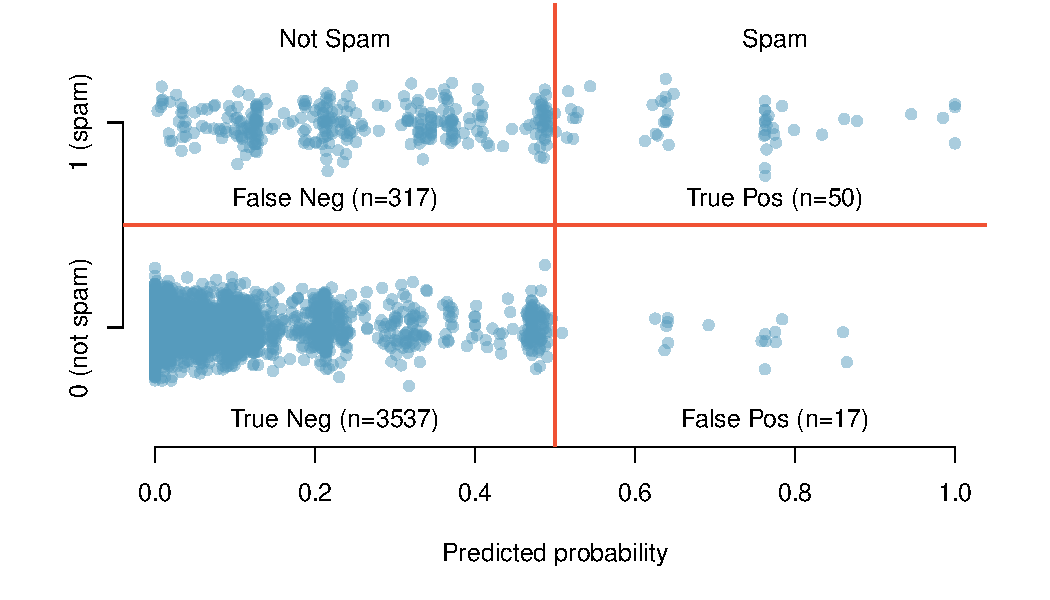
\includegraphics[width=0.9\textwidth]{9-5_logistic_reg/figures/spam/spam5-3.pdf}}
\only<4|handout:0>{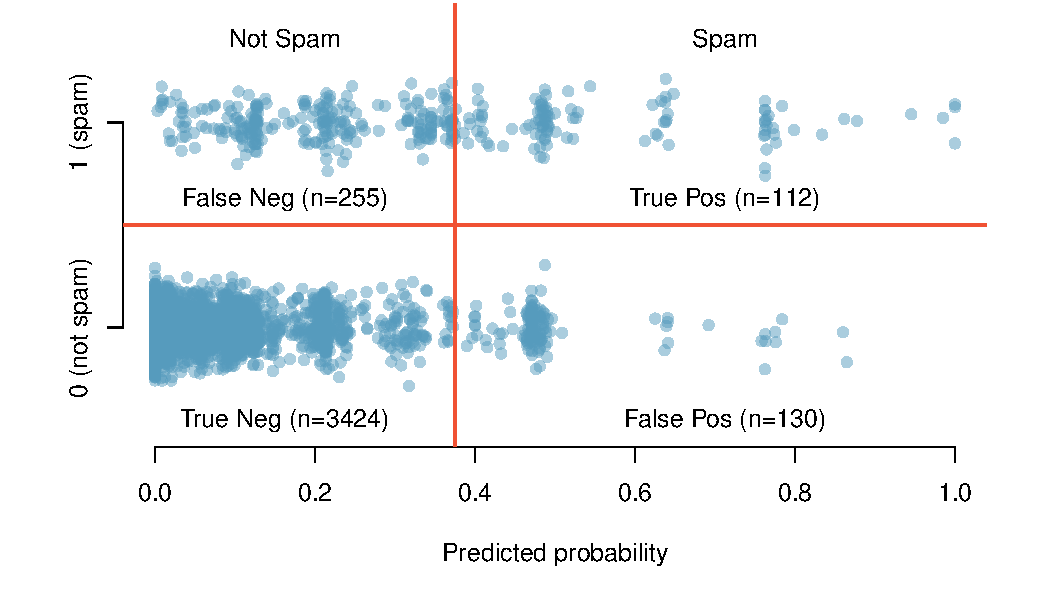
\includegraphics[width=0.9\textwidth]{9-5_logistic_reg/figures/spam/spam5-4.pdf}}
\only<5|handout:0>{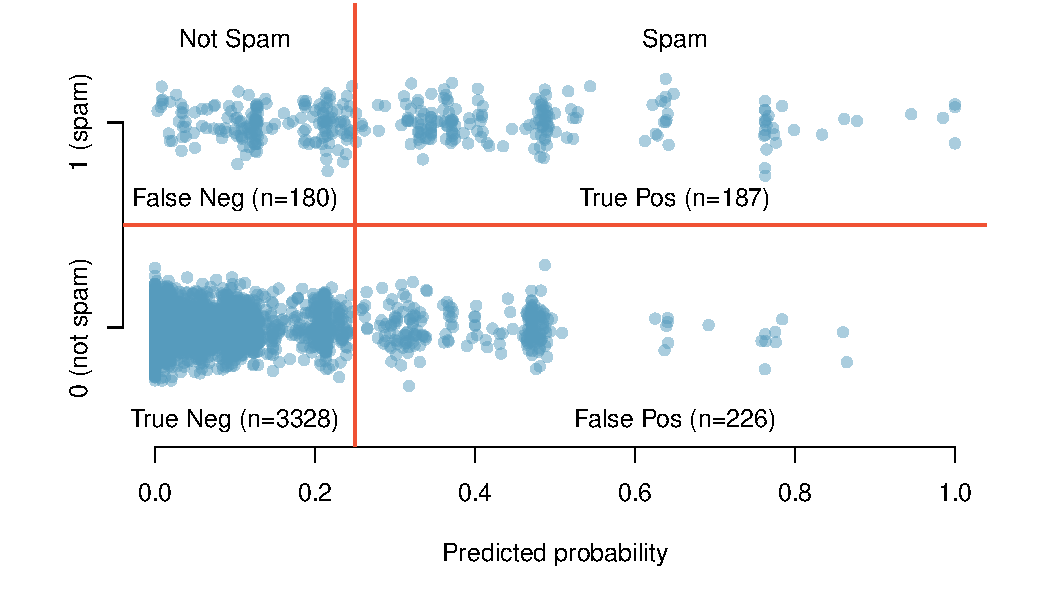
\includegraphics[width=0.9\textwidth]{9-5_logistic_reg/figures/spam/spam5-5.pdf}}
\end{center}

{\footnotesize
\begin{center}
\begin{tabular}{|c|ccccc|}
\hline
Threshold   & 0.75 & 0.625 & 0.5 & 0.375 & 0.25 \\
\hline
Sensitivity & 0.074 & \only<2->{0.106} & \only<3->{0.136} & \only<4->{0.305} & \only<5->{0.510} \\
Specificity & 0.997 & \only<2->{0.995} & \only<3->{0.995} & \only<4->{0.963} & \only<5->{0.936} \\
\hline
\end{tabular}
\end{center}
}

\end{frame}


%%%%%%%%%%%%%%%%%%%%%%%%%%%%%%%%%%

\begin{frame}
\frametitle{Relationship between Sensitivity and Specificity}

{\footnotesize
\begin{center}
\begin{tabular}{|c|ccccc|}
\hline
Threshold   & 0.75 & 0.625 & 0.5 & 0.375 & 0.25 \\
\hline
Sensitivity & 0.074 & 0.106 & 0.136 & 0.305 & 0.510 \\
Specificity & 0.997 & 0.995 & 0.995 & 0.963 & 0.936 \\
\hline
\end{tabular}
\end{center}
}


\begin{center}
\only<1|handout:0>{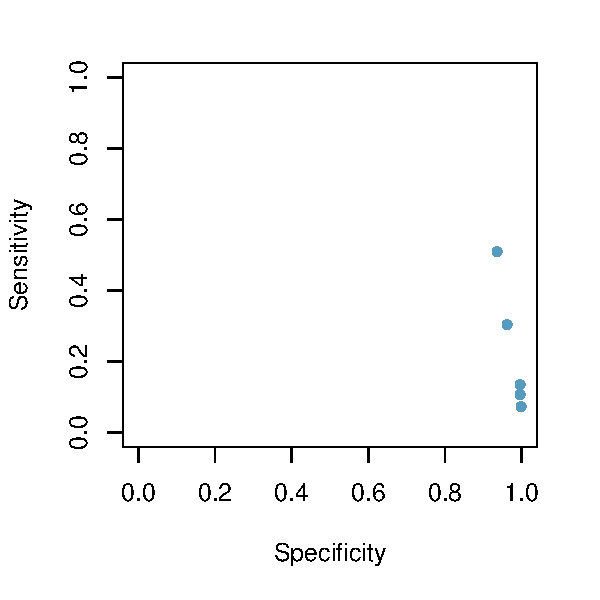
\includegraphics[width=0.5\textwidth]{9-5_logistic_reg/figures/spam/sen_vs_spec1.pdf}}
\only<2|handout:0>{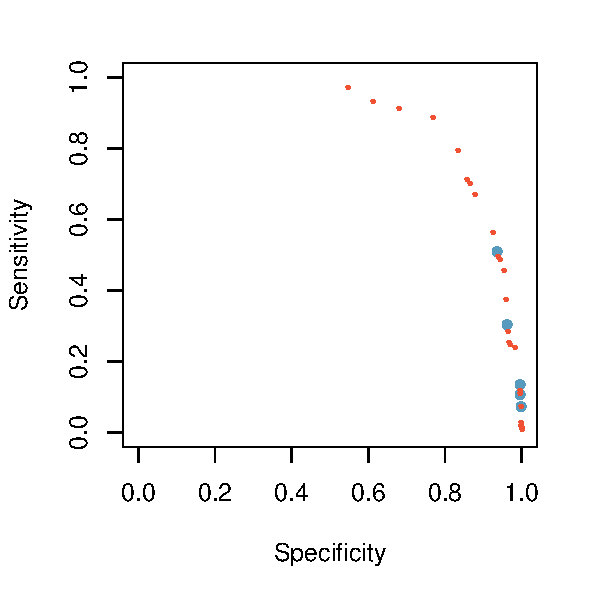
\includegraphics[width=0.5\textwidth]{9-5_logistic_reg/figures/spam/sen_vs_spec2.pdf}}
\only<3|handout:1>{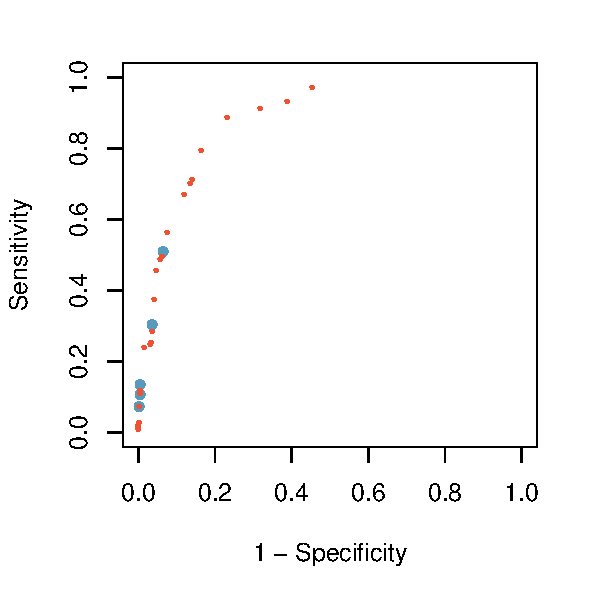
\includegraphics[width=0.5\textwidth]{9-5_logistic_reg/figures/spam/sen_vs_spec3.pdf}}
\end{center}

\end{frame}

%%%%%%%%%%%%%%%%%%%%%%%%%%%%%%%%%%

\begin{frame}
\frametitle{Receiver operating characteristic (ROC) curve}

\vspace{-8mm}

\begin{center}
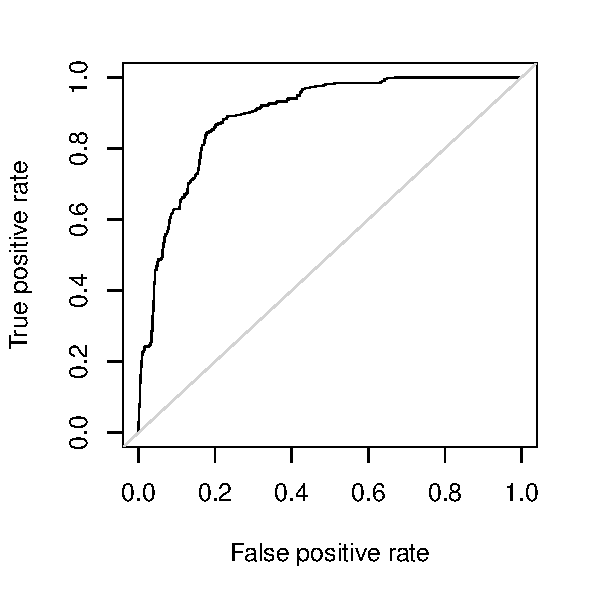
\includegraphics[width=0.7\textwidth]{9-5_logistic_reg/figures/spam/ROC.pdf}
\end{center}

\end{frame}

%%%%%%%%%%%%%%%%%%%%%%%%%%%%%%%%%%

\begin{frame}
\frametitle{Receiver operating characteristic (ROC) curve (cont.)}

Why do we care about ROC curves?

\begin{itemize}
\item Shows the trade off in sensitivity and specificity for all possible thresholds.

\item Straight forward to compare performance vs. chance.

\item Can use the area under the curve (AUC) as an assessment of the predictive ability of a model.

\end{itemize}

\end{frame}

%%%%%%%%%%%%%%%%%%%%%%%%%%%%%%%%%%

\begin{frame}[fragile]
\frametitle{Refining the Spam model}

\vspace{-5mm}

{\footnotesize
\begin{verbatim}
g_refined = glm(spam ~ to_multiple+cc+image+attach+winner
                      +password+line_breaks+format+re_subj
                      +urgent_subj+exclaim_mess, 
                data=email, family=binomial)
summary(g_refined)
\end{verbatim}

\begin{center}
\begin{tabular}{rrrrr}
  \hline
 & Estimate & Std. Error & z value & Pr($>$$|$z$|$) \\ 
  \hline
(Intercept) & -1.7594 & 0.1177 & -14.94 & 0.0000 \\ 
  to\_multipleyes & -2.7368 & 0.3156 & -8.67 & 0.0000 \\ 
  ccyes & -0.5358 & 0.3143 & -1.71 & 0.0882 \\ 
  imageyes & -1.8585 & 0.7701 & -2.41 & 0.0158 \\ 
  attachyes & 1.2002 & 0.2391 & 5.02 & 0.0000 \\ 
  winneryes & 2.0433 & 0.3528 & 5.79 & 0.0000 \\ 
  passwordyes & -1.5618 & 0.5354 & -2.92 & 0.0035 \\ 
  line\_breaks & -0.0031 & 0.0005 & -6.33 & 0.0000 \\ 
  formatPlain & 1.0130 & 0.1380 & 7.34 & 0.0000 \\ 
  re\_subjyes & -2.9935 & 0.3778 & -7.92 & 0.0000 \\ 
  urgent\_subjyes & 3.8830 & 1.0054 & 3.86 & 0.0001 \\ 
  exclaim\_mess & 0.0093 & 0.0016 & 5.71 & 0.0000 \\ 
   \hline
\end{tabular}
\end{center}

}
\end{frame}

%%%%%%%%%%%%%%%%%%%%%%%%%%%%%%%%%%

\begin{frame}[fragile]
\frametitle{Comparing models}

\vspace{-8mm}

\begin{center}
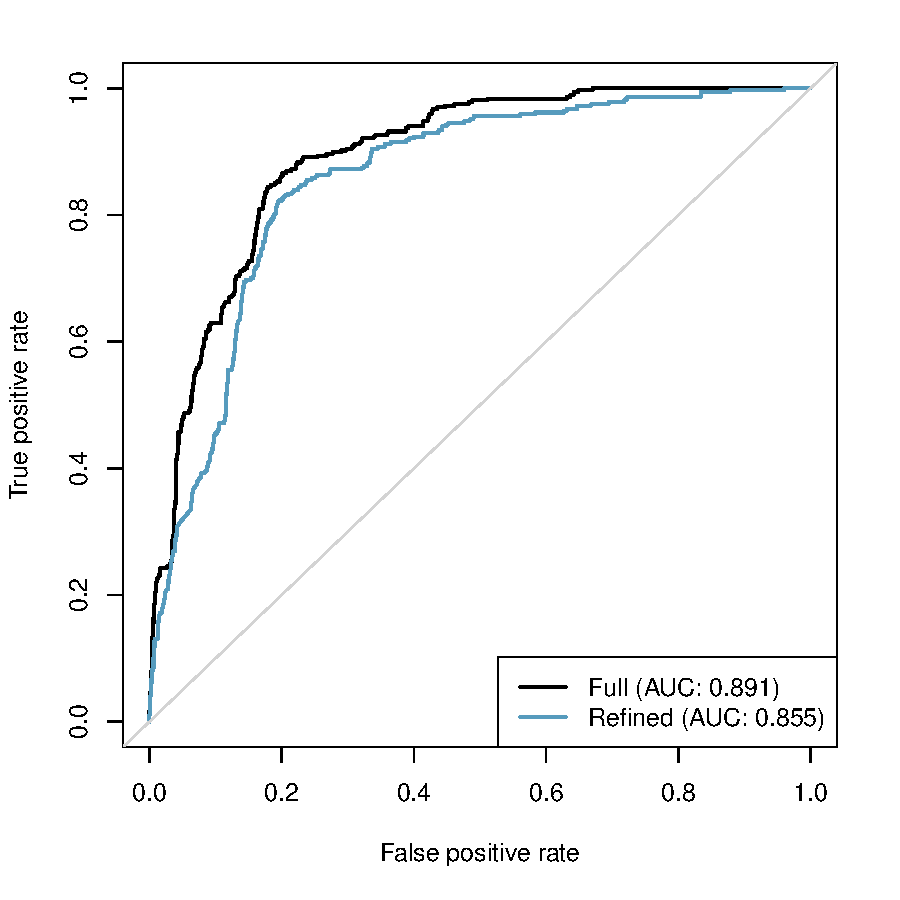
\includegraphics[width=0.7\textwidth]{9-5_logistic_reg/figures/spam/ROC_comp.pdf}
\end{center}

\end{frame}

%%%%%%%%%%%%%%%%%%%%%%%%%%%%%%%%%%

\subsection{Utility Functions}

%%%%%%%%%%%%%%%%%%%%%%%%%%%%%%%%%%%

\begin{frame}
\frametitle{Utility Functions}

There are many other reasonable quantitative approaches we can use to decide on what is the ``best'' threshold.\\
~\\
If you've taken an economics course you have probably heard of the idea of utility functions, we can assign costs and benefits to each of the possible  outcomes and use those to calculate a utility for each circumstance.

\end{frame}

%%%%%%%%%%%%%%%%%%%%%%%%%%%%%%%%%%

\begin{frame}
\frametitle{Utility function for our spam filter}

To write down a utility function for a spam filter we need to consider the costs / benefits of each out.

\begin{center}
 \renewcommand\arraystretch{1.5}
\begin{tabular}{l|c}
Outcome & Utility \\
\hline
True Positive  & \only<2->{1} \\
True Negative  & \only<3->{1} \\
False Positive & \only<4->{-50} \\
False Negative & \only<5->{-5} \\
\end{tabular}
\end{center}
~\\
\only<6>{
\[U(p) = TP(p) + TN(p) - 50 \times FP(p) - 5 \times FN(p)\]
}

\end{frame}

%%%%%%%%%%%%%%%%%%%%%%%%%%%%%%%%%%

\begin{frame}
\frametitle{Utility for the 0.75 threshold}

For the email data set picking a threshold of 0.75 gives us the following results:
\vspace{-1.5mm}
\begin{align*}
FN = 340 &\qquad TP = 27 \\
TN = 3545 &\qquad FP = 9
\end{align*}

\pause

\begin{align*}
U(p) &= TP(p) + TN(p) - 50 \times FP(p) - 5 \times FN(p) \\
     &= 27+3545-50\times9-5\times340 = 1422
\end{align*}

\pause

Not useful by itself, but allows us to compare with other thresholds.

\end{frame}

%%%%%%%%%%%%%%%%%%%%%%%%%%%%%%%%%%

\begin{frame}
\frametitle{Utility curve}

\vspace{-5mm}

\begin{center}
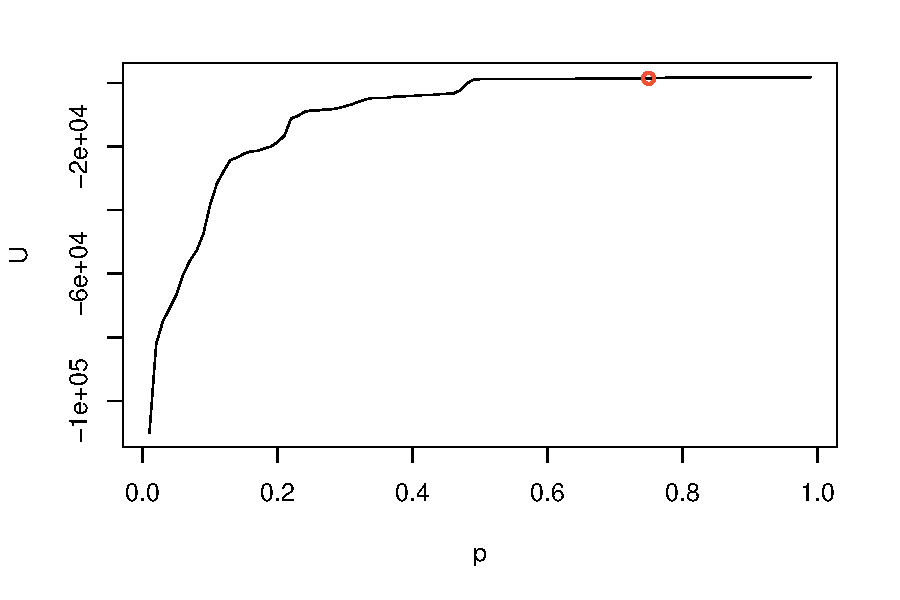
\includegraphics[width=\textwidth]{9-5_logistic_reg/figures/spam/utility.pdf}
\end{center}

\end{frame}


%%%%%%%%%%%%%%%%%%%%%%%%%%%%%%%%%%

\begin{frame}
\frametitle{Utility curve (zoom)}

\vspace{-5mm}

\begin{center}
\only<1|handout:0>{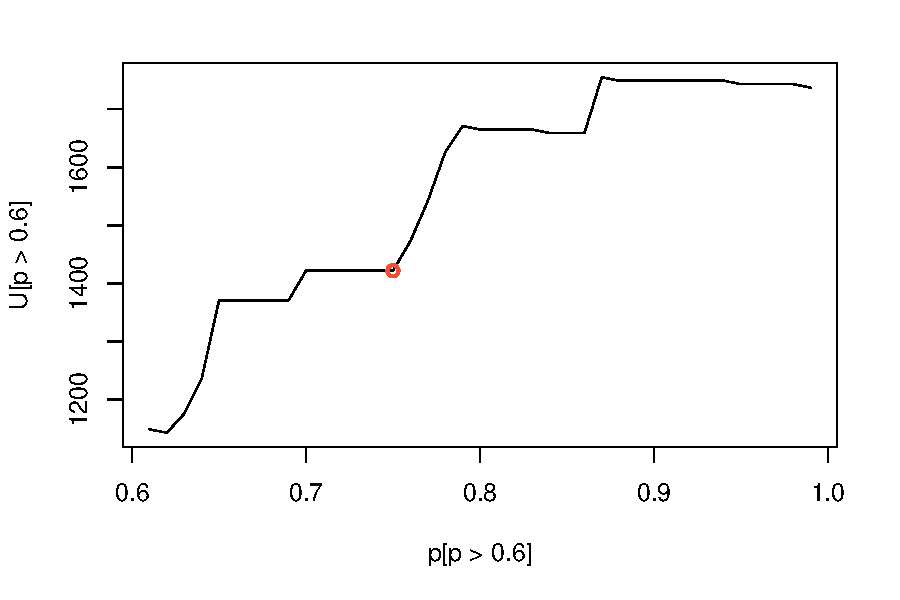
\includegraphics[width=\textwidth]{9-5_logistic_reg/figures/spam/utility2.pdf}}
\only<2|handout:1>{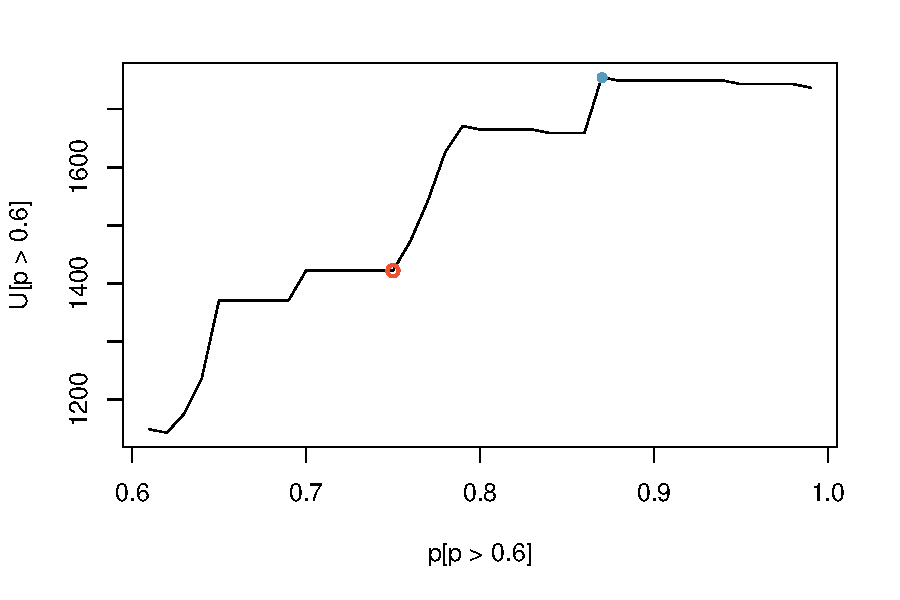
\includegraphics[width=\textwidth]{9-5_logistic_reg/figures/spam/utility3.pdf}}
\end{center}

\end{frame}

%%%%%%%%%%%%%%%%%%%%%%%%%%%%%%%%%%

\begin{frame}
\frametitle{Maximum Utility}

\begin{center}
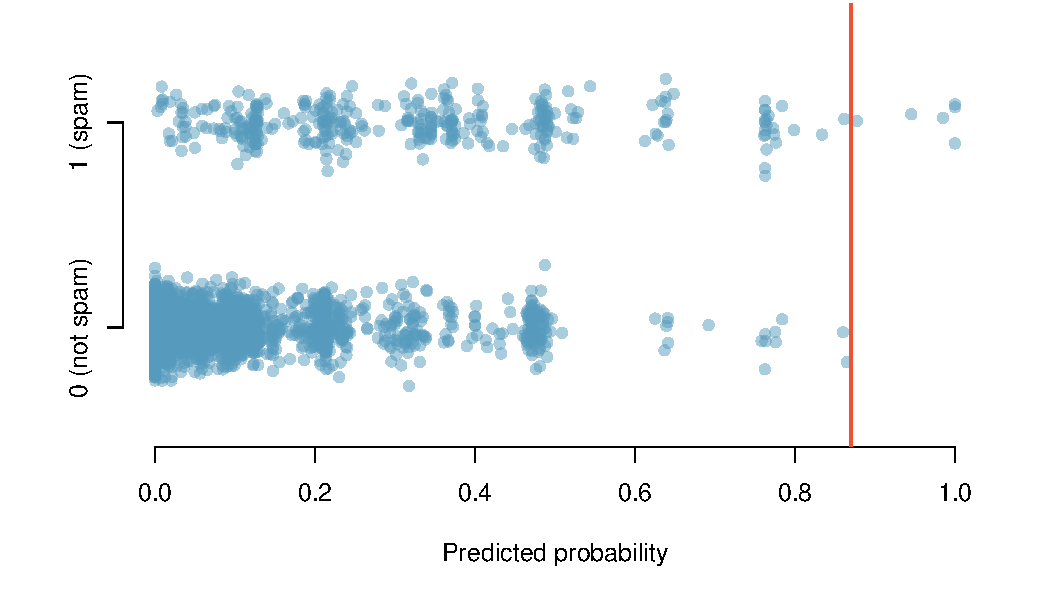
\includegraphics[width=\textwidth]{9-5_logistic_reg/figures/spam/utility4.pdf}
\end{center}

\end{frame}


\end{document}


\end{frame}



%%%%%%%%%%%%%%%%%%%%%%%%%%%%%%%%%%%%
% End document
%%%%%%%%%%%%%%%%%%%%%%%%%%%%%%%%%%%%

\end{document}